\setmainfont{Noto Serif}
\setsansfont{Noto Sans}
\setmonofont{Noto Sans Mono}
\setstretch{1.35}


%\phantomsection
\section{Описание электронного строения атомов и молекул}
%\addcontentsline{toc}{chapter}{1 Описание электронного строения атомов и молекул}
%\markboth{Описание электронного строения атомов и молекул}{Описание электронного строения атомов и молекул}
\subsection{Угловой момент. Сложение моментов}
1. Прямой расчет дает $\braket{\widehat{V}}= -\frac{q_e^2}{4\pi \varepsilon a_0}=-2\braket{ \widehat{K}}=2\braket {\widehat{H}}$, где $\varepsilon_0$ – электрическая постоянная, $a_0$ – радиус Бора. \par
2. Энергия уровней в атоме H равна $E_n = -\frac{\mu q_e^4}{32 \pi^2 \epsilon_0^2 \hbar^2}\frac{1}{n^2}$, где $\mu=\frac{m_N m_e}{m_N + m_e}$ – приведенная масса ядра атома и электрона. Учитывая, что $m_D = 2m_H$, а также пренебрегая малой массой электрона в знаменателе дроби, можно получить: $\Delta E \approx E_0 ( \frac{m_em_H}{2m_H^2} ) = E_0 (\frac{m_e}{2m_H}) \approx -3,703\cdot 10^{-3}$ эВ, где $E_0 = -\frac{ m_e q_e^4}{32 \pi^2 \epsilon_0^2 \hbar^2}$, $q_e$ – заряд электрона, $\varepsilon_0$ – электрическая постоянная.\par
3. Используя базис полного момента гамильтониан можно переписать следующим образом: $\widehat{H}=\frac{a}{2}( {F}^2 -{S}^2-{I}^2)$, где $F$ – полный спин системы. Энергия данного гамильтониана зависит только от значения $F$, которое для системы двух спинов 1/2 равно 1, 0. Таким образом основное состояние расщепляется на два уровня энергии: $E_{11}=E_{10}=E_{1-1}=a/4$; $E_{00}=-3a/4$, где первый индекс в обозначении энергетических уровней равен $F$, второй – $m_F$. Полные волновые функции могут быть записаны в виде $\ket {n\,l\,m\,F\,m_F\,S\,I}=\ket{F\,m_F}$, а именно: $\ket{ 1\, 0\, 0\,  1\, 1\, \frac{1}{2}\, \frac{1}{2}} = \ket{1\,1} = \ket{1s}\alpha{\alpha}_N$, $\ket{1\,0} = \ket{1s}\frac{1}{\sqrt{2}}(\alpha{\beta}_N +{\beta}{\alpha}_N)$; $\ket{1\,-1} = \ket{1s}\beta{\beta}_N$; $\ket{0\,0} = \ket{1s}\frac{1}{\sqrt{2}}(\alpha{\beta}_N - {\beta}{\alpha}_N)$, где $\ket{1s} = R_{10}\textit{Y}_{00}.$\par
4. Когда протон прилипает к ядру атома водорода, то образуется ядро $^2_2\text{He}^+$. Далее нужно выполнить разложение волновой функции состояния $1s$ атома He по состояниям атома водорода: $\ket{1s}_{He} = a\ket{1s}_{H} + b\ket{2s}_H + c\ket{2p_0}_H + \ldots$. Таким образом нам требуется найти квадрат коэффициента перед первым слагаемым в данном разложении: $W_{1s}={|\braket{1s_H|1s_{He}}|}^2$. Необходимые для расчета волновые функции – это функции водородоподобного атома:\par
\vspace{-\parskip+1mm}
$\ket{1s}_{H}=\sqrt{\frac{1}{\pi a^3_H}}\exp(-r/a_H)$;\quad $\ket{1s}_{He}=\sqrt{\frac{2^3}{\pi a^3_{He}}}\exp(-2r/a_{He})$,\par
\vspace{-\parskip+1mm}
где $a_{\mu}=\frac{m_e}{\mu}a_0$, где $a_0$ – радиус Бора, $m_e$ – масса электрона, $\mu$ – приведенная масса системы электрон-ядро. Расчет показывает, что искомый интеграл равен:\par
\vspace{-\parskip+2mm}
$W_{1s}=\left(\sqrt{\dfrac{8}{a_H^3 a_{He}^3}}\dfrac{8}{\left(\frac{2}{a_{He}}+\frac{1}{a_H}\right)^3}\right)^2 = 0,702$. \par
5. Одноэлектронные волновые функции в атоме называются атомными орбиталями. Для облегчения визуализации обычно вводится базис вещественных линейных комбинаций сферических гармоник, который будет соответствовать $s, p, d, f$ и т. д. орбиталям. Одним из способов визуализации атомных орбиталей является построение контурных диаграмм. В них приводят поверхности одинаковой вероятности найти электрон в некоторой области пространства. Обычно изображают только одну поверхность, соответствующую вероятности $90\%$. Дополнительно знак волновой функции или, другими словами, фазу обозначают цветом или знаками $+/-$. Контурные диаграммы вещественных комбинаций сферических гармоник до $l = 2$ приведены на рисунке. При умножении на~соответствующую радиальную волновую функцию они дадут $ns, np, nd$ атомные орбитали.\par
\vspace{-\parskip}
\vspace{0mm}
\begin{figure}[h]
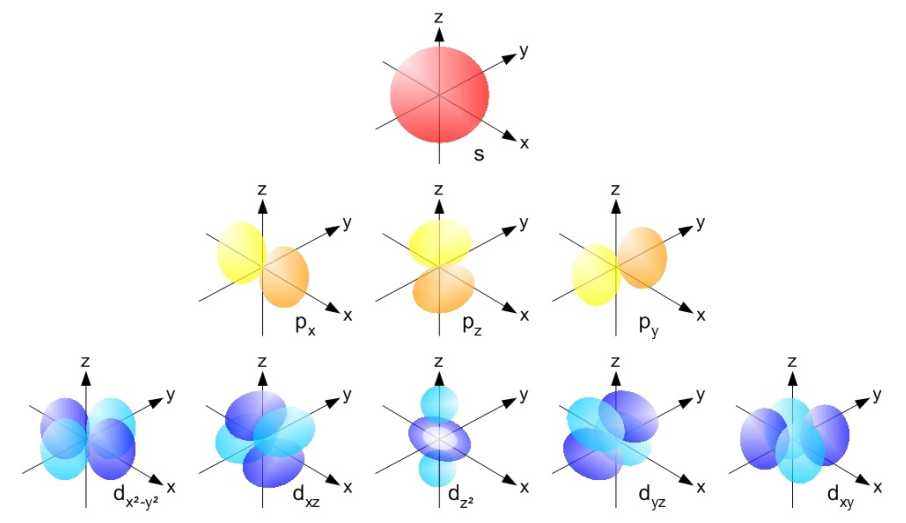
\includegraphics[width=6.0cm]{images/Fig_1_1_4_dec.png}
\centering
\end{figure}
\vspace{-\parskip}
\vspace{2mm}
\par
6. $N_S = 2S^2+3S+1$; $N_A= 2S^2+S$.\par
7. Связь базисов $\ket{L M_L}$ и $\ket{L_1 m_{L_1}}\ket{L_2 m_{L_2}}$:\par
\vspace{-\parskip+1mm}
$\ket{2\pm2}=\ket{1\pm1}\!\ket{1\pm1};$\quad $\ket{2\pm1} = \frac{1}{\sqrt2}(\ket{10}\!\ket{1\pm1} + \ket{1\pm1}\!\ket{10});$\par
\vspace{-\parskip+1mm}
$\ket{20} = \frac{1}{\sqrt6}(\ket{1-1}\!\ket{11} + 2\ket{10}\!\ket{10}+\ket{11}\!\ket{1-1});$\par
\vspace{-\parskip+1mm}
$\ket{1\pm1} = \frac{1}{\sqrt2}(\ket{10}\!\ket{1\pm1} - \ket{1\pm1}\!\ket{10});$\quad$\ket{10} = \frac{1}{\sqrt2}(\ket{1-1}\!\ket{11} - \ket{11}\!\ket{1-1});$\par
\vspace{-\parskip+1mm}
$\ket{00} = \frac{1}{\sqrt3}(\ket{1-1}\!\ket{11} - \ket{10}\!\ket{10}+\ket{11}\!\ket{1-1}).$\par
\vspace{-\parskip+1mm}
Вероятности $W_J$ обнаружить различные значения полного момента $J$: $W_{2} = 2/3$, $W_{1} = 0$, $W_{0} = 1/3$.
%\hspace{\fill}
\par
8. $2L_2+1$.\par
9. Количество состояний с определенными проекциями полного момента для~системы из $N$ электронов подчиняется биномиальному распределению. Любой возможный полный спин системы $K$ имеет нулевую проекцию. Всего нулевых проекций $C_{N}^{\,N/2}$. Любой возможный полный спин системы $K>0$ имеет проекцию равную 1. Всего единичных проекций $C_{N}^{\,(N+2)/2}$. Тогда $K=0$ в данной системе встретится $C_{N}^{\,N/2} - C_{N}^{\,(N+2)/2}$ раз. В случае нечетного $N$ задача решается аналогично, только минимальный возможный полный спин системы равен 1/2, то есть каждый полный спин $K$ имеет проекцию $1/2$. \par
10. $\widehat{S}_-=\begin{pmatrix}
0 & 0 & 0 & 0 & 0 & 0 \\
\sqrt{5} & 0 & 0 & 0 & 0 & 0\\
0 & 2\sqrt{2} & 0 & 0 & 0 & 0\\
0 & 0 & 3 & 0 & 0 & 0\\
0 & 0 & 0 & 2\sqrt{2} & 0 & 0\\
0 & 0 & 0 & 0 & \sqrt{5} & 0\\
\end{pmatrix}$
\par
11. $(\vec{S}_1,\vec{S}_2)=\frac{1}{2}( J^2 - S_1^2-S_2^2)$, где $J$ – полный спин системы. Средние значения равны $1/4$ и $-3/4$ для триплетного и синглетного состояния, соответственно.\par
12. $n^2.$\par
13. Задача 1 контрольной работы 1 осеннего семестра 2023/2024 учебного года. Систему можно обнаружить в состояниях с полным моментом $J_1=S_1+S_2$ и $J_2=S_1+S_2-1$ с вероятностями $W_1=\frac{S_1}{S_1+S_2}$; $W_2=\frac{S_2}{S_1+S_2}$. Среднее значение квадрата полного момента равно $\braket{S^2}=(S_1+S_2 )^2+S_1-S_2$.
\par
14. $3S^2-4n^2+3S+1$, если $S$ и $n$ – целые числа.\par
15. Для данного состояния могут реализоваться два значения полного спина $2N$ и $2N-1$ с вероятностями $W_{N}=\frac{1}{2N}$; $W_{N-1}=\frac{2N-1}{2N}$.\par
16. $\ket{\frac{3}{2}\,\frac{3}{2}}=\alpha\alpha\alpha$;\hspace{\fill}
$\ket{\frac{3}{2}\,\frac{1}{2}}=\frac{1}{\sqrt3}( \beta\alpha\alpha+\alpha\beta\alpha +\alpha\alpha\beta);$\hspace{\fill}$\ket{\frac{3}{2}\,-\!\frac{1}{2}}=\frac{1}{\sqrt3}( \alpha\beta\beta +\beta\alpha\beta +\beta\beta\alpha);$\par
\vspace{-\parskip+1mm}
$\ket{\frac{3}{2}\,-\!\frac{3}{2}}=\beta\beta\beta$. \hspace{\fill} $\ket{\frac{1}{2}\,\frac{1}{2}}_1 = \frac{1}{\sqrt2}( \beta\alpha\alpha-\alpha\beta\alpha);$ \hspace{\fill} $\ket{\frac{1}{2}\,\frac{1}{2}}_2 = \frac{1}{\sqrt6}( \beta\alpha\alpha+\alpha\beta\alpha -2\alpha\alpha\beta)$;\par
\vspace{-\parskip+1mm}
$\ket{\frac{1}{2}\,-\!\frac{1}{2}}_1 = \frac{1}{\sqrt2}( \alpha\beta\beta-\beta\alpha\beta);$ \quad $\ket{\frac{1}{2}\,-\!\frac{1}{2}}_2 = \frac{1}{\sqrt6}( \alpha\beta\beta+\beta\alpha\beta -2\beta\beta\alpha)$.
\par
17. Количество состояний с определенными проекциями полного момента для~системы из $N$ электронов подчиняется биномиальному распределению. Для~проекции $M =N/2-k$ количество состояний равно $C_{N}^{\,N/2-M}=C_{N}^{\,k}$. Альтернативно можно воспользоваться треугольником Паскаля:\par
\vspace{0.7mm}
\Longstack[l]{
%N=0\\
N=1\\
N=2\\
N=3\\
N=4\\
N=5\z \\
%M\qquad\ \\
}\hspace{\fill}
\Longstack{
1\x 1\\
1\x 2\x 1\\
1\x 3\x 3\x 1\\
1\x 4\x 6\x 4\x 1\\
1\x 5\y\, 10\z\, 10\y\, 5\quad\,\,\,\,\, 1\\
}\quad\quad
\Longstack{
1\x 1 \x 1\\
1\x 2\x 3\x 2\x 1\\
1\x 3\x 6\x 7\x 6\x 3\x 1\\
1\x 4\y 10\z 16\z 19\z 16\z 10\y 4\x 1\\
1\x 5\y 15\z 30\z 45\z 51\z 45\z 30\z 15\y 5\x 1\\
}
\vspace{-\parskip}
\\
Система частиц с моментом $\geq1$ описывается мультиномиальным распределением. Его можно визуализировать с использованием обобщенного треугольника Паскаля, который для момента 1 приведен выше. Количество состояний с~определенными проекциями полного момента будет определяться мультиномиальными коэффициентами.\par
18. Задача 2 контрольной работы 1 осеннего семестра 2024/2025 учебного года. (1) Полная волновая функция – антисимметрична: $\frac{1}{\sqrt{2}}(\phi_1\phi_2-\phi_2\phi_1)\ket{T_{0,\,\pm1}};$ $\frac{1}{\sqrt{2}}(\phi_1\phi_2+\phi_2\phi_1)\ket{S_{0}},$ где $\ket{T_{0,\,\pm1}}$ и $\ket{S_{0}}$ – триплетные и синглетные спиновые волновые функции, соответственно, $\phi_1, \phi_2$ – орбитальные волновые функции. (2)~Полную волновую функцию можно не антисимметризовать: $\phi_1\phi_2\alpha\alpha$, $\phi_1\phi_2\alpha\beta$, $\phi_1\phi_2\beta\alpha$, $\phi_1\phi_2\beta\beta$. (3) Полная волновая функция должна быть симметрична относительно перестановки, тогда: $\frac{1}{\sqrt{2}}(\phi_1\phi_2+\phi_2\phi_1)\ket{2\,M_S};$ $\frac{1}{\sqrt{2}}(\phi_1\phi_2-\phi_2\phi_1)\ket{1\,M_S};$ $\frac{1}{\sqrt{2}}(\phi_1\phi_2+\phi_2\phi_1)\ket{0\,0},$ где $\ket{2\, M_S}$, $\ket{1\, M_S}$, $\ket{0\, M_S}$ – соответствующие спиновые волновые функции для полного спина $S=2,1,0$, см. задачу 1.7. Частицы можно считать различимыми, если они расположены на большом расстоянии друг от~друга, по~сравнению с их областью делокализации, то есть если их волновые функции не перекрываются.\par
19. Матричные элементы равны 24, $-3$, $-9$, соответственно.\par
20. Задачу можно решить прямым расчетом интеграла $\braket{\psi|{S}^2|\psi}$, используя равенства ${S}^2 = (\vec{S},\,\vec{S})=S_{z}S_{z}+S_{y}S_{y}+S_{x}S_{x}$, $S_x=(S_+ + S_-)/2$, $S_y=(S_+ - S_-)/2i$. Расчет дает $\braket{{S}^2} = n^2 - nN + \frac{1}{4}N(N+2)$.\par
\newpage

\subsection{Термы многоэлектронных атомов}
1. В пределе LS связи для данной электронной конфигурации реализуются термы: $^4S$, $^2D$, $^2P$. При учете слабого спин-орбитального взаимодействия возникают мультиплеты:  $^4S_{\frac32}$, $^2D_{\frac52,\,\,\frac32}$, $^2P_{\frac32,\,\,\frac12}$.\par
2. Основной терм $^4I$, основной мультилет $^4I_{\frac92}$.\par
3. Термы: $1 \times \,^2G$, $ 3 \times \,^2F$, $ 5 \times \,^2D$, $ 6 \times \,^2P$, $ 2 \times \,^2S$, $1 \times \,^4F$, $ 3 \times \,^4D$, $ 3 \times \,^4P$, $ 2 \times \,^4S$, $1 \times \, ^6P$. Мультиплеты: $1 \times \,^2G_{\frac92,\,\frac72}$, $ 3 \times \,^2F_{\frac72,\,\frac52}$, $ 5 \times \,^2D_{\frac52,\,\frac32}$, $ 6 \times \,^2P_{\frac32,\,\frac12}$, $ 2 \times \,^2S_{\frac12}$, $1 \times \,^4F_{\frac92,\,\frac72,\,\frac52,\,\frac32}$, \par
\vspace{-\parskip+1.3mm}
$ 3 \times \,^4D_{\frac72,\,\frac52,\,\frac32,\,\frac12}$, $ 3 \times \,^4P_{\frac52,\,\frac32,\,\frac12}$, $ 2 \times \,^4S_{\frac32}$, $1 \times \,^6P_{\frac72,\,\frac52,\,\frac32}$.\par
4. Основной терм $^{n+1}\left[\frac n2 (2l-n+1)\right]$.\par
5. Основной терм $^{3}\left[ 2l+1 \right]$. Общее число термов $N_{\Sigma}=2l+1$. Триплетных термов $N_{\text{T}}=l$. Синглетных термов $N_{\text{S}}=l+1$.\par
\begin{wrapfigure}{r}{38mm} %this figure will be at the right
    \centering
    \vspace{-2mm}
    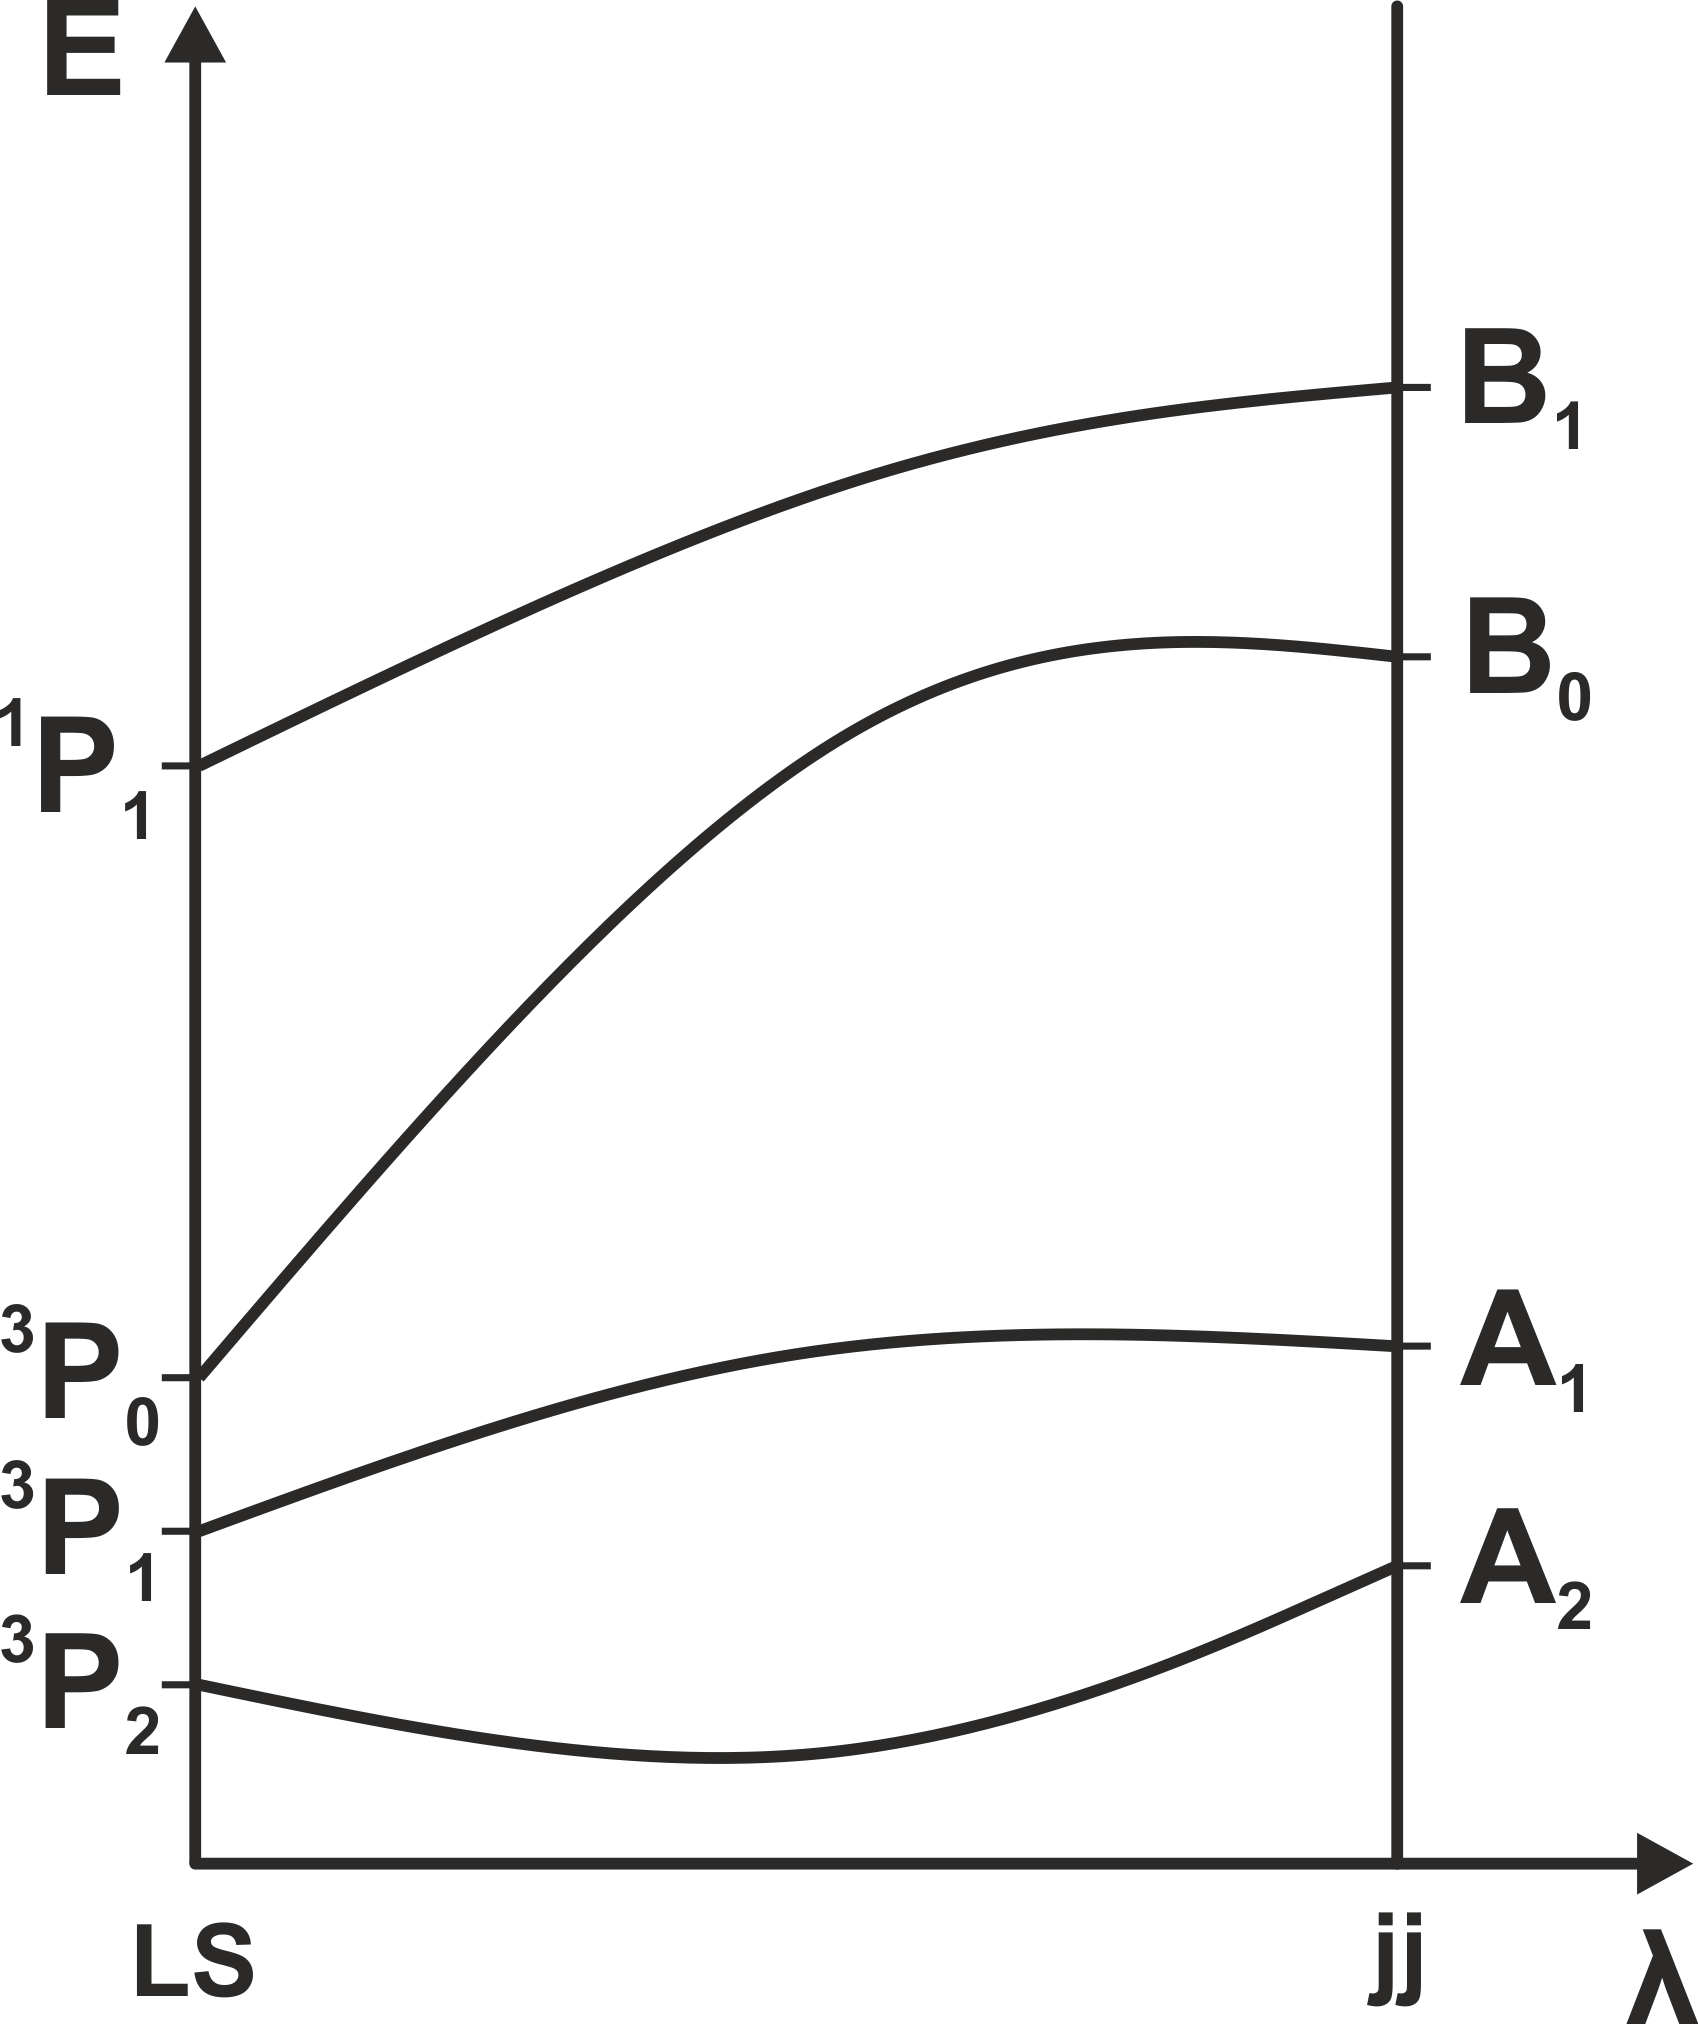
\includegraphics[width=30mm]{images/Fig_1_2_6_dec.png}
    \vspace{-3mm}
\end{wrapfigure}
6. Мультиплеты данной конфигурации в пределе LS\hspace{\fill}связи:\hspace{\fill}$^3P_{2,\,1,\,0}$,\hspace{\fill}$^3P_{1}$;\hspace{\fill}в\hspace{\fill}пределе\hspace{\fill}jj\hspace{\fill}связи:\par
\vspace{-\parskip+1mm}
$\Big( \frac32\,\,\frac32\,\,\frac32\,\,\frac12\,\,\frac12\,\,\frac12 \Big)_{2,\,1}$,\hspace{\fill}$\Big( \frac32\,\,\frac32\,\,\frac32\,\,\frac32\,\,\frac12\,\,\frac12 \Big)_{1,\,0}$.\hspace{\fill}Мультиплеты\par
\vspace{-\parskip+1mm}
коррелируют по величине полного момента $J$. Состояния с одинаковой симметрией (с одинаковым $J$) пересекаться не могут. Качественная корреляционная диаграмма приведена на рисунке. Реализующиеся состояния для случайя jj связи для удобства обозначены $A_{2,\,1}$ и $B_{1,\,0}$. При решении задачи можно также использовать эквивалентную электронную конфигурацию $p^1s^1$, если в ней корректно учесть изменение знака эффективной константы спин-орбитального взаимодействия $\lambda$, при неизменных знаках одноэлектронных констант спин-орбитального взаимодействия $\xi_i$. \par
7. Функция принадлежит электронной конфигурации $n_1p^1n_2d^1$ и терму $^3F$.\par
8. В пределе jj связи для данной электронной конфигурации реализуются термы: $\Big( \frac32\,\,\frac32\,\,\frac32 \Big)_{\frac32}$, $\Big( \frac12\,\,\frac32\,\,\frac32 \Big)_{\frac52,\,\frac32,\,\frac12}$, $\Big( \frac12\,\,\frac12\,\,\frac32 \Big)_{\frac32}$. Последний терм является основным.\par
9. В данном случае термы можно найти используя антисимметричность полной волновой функции относительно перестановки тождественных электронов. Полная волновая функция представляет собой произведение спиновой и орбитальной части, симметрия каждой из которых чередуется начиная с~симметричного поведения для максимального момента. Итого реализуются термы: $^1N$, $^1L$, $^1I$, $^1G$, $^1D$, $^1S$, $^3M$, $^3K$, $^3H$, $^3F$, $^3P$.\par
10. Задача 1 дифференциального зачета осеннего семестра 2023/2024 учебного года. Используя правило интервалов Ланде можно определить 4 величины $\lambda$~равные $-104$ см$^{-1}$, $-96$ см$^{-1}$, $-92$ см$^{-1}$, $-90$ см$^{-1}$. Отсюда $\overline \lambda = -95,5$ см$^{-1}$.\par
11. Основной терм $^4S$. Волновые функции, обозначаемые $\ket{L\,M_L;\,S\,M_S}$, являются произведением орбитальной и спиновой части. Орбитальная часть имеет вид: $\psi_0=\frac{1}{\sqrt6}(\phi_1\phi_0\phi_{-1} + \phi_0\phi_{-1}\phi_{1} + \phi_{-1}\phi_1\phi_{0} - \phi_{-1}\phi_0\phi_{1} - \phi_1\phi_{-1}\phi_{0} - \phi_0\phi_1\phi_{-1} )$, где $\phi_1 = \textit{Y}_{11}$, $\phi_0 = \textit{Y}_{10}$, $\phi_{-1} = \textit{Y}_{1-1}$. Спиновая часть, см. также задачу 1.1.16, имеет вид: $\xi_{\frac32}=\alpha \alpha \alpha$, \par
\vspace{-\parskip+0.8mm}
$\xi_{\frac12}=\frac{1}{\sqrt3} (\beta \alpha \alpha + \alpha \beta \alpha + \alpha \alpha \beta )$,\hspace{\fill}$\xi_{-\frac12}=\frac{1}{\sqrt3} (\alpha \beta \beta + \beta \alpha \beta + \beta \beta \alpha )$,\hspace{\fill}$\xi_{-\frac32}=\beta \beta \beta$.\hspace{\fill}Волновые \par
\vspace{-\parskip+1.2mm}
функции\hspace{\fill}основного\hspace{\fill}терма\hspace{\fill}$\ket{0\,0;\,\frac32\,\frac32}=\psi_0 \xi_{\frac32}$,\hspace{\fill}$\ket{0\,0;\,\frac32\,\frac12}=\psi_0 \xi_{\frac12}$, $\ket{0\,0;\,\frac32\,-\!\frac12}=\psi_0 \xi_{-\frac12}$, \par
\vspace{-\parskip+1mm}
$\ket{0\,0;\,\frac32\,-\!\frac32}=\psi_0 \xi_{-\frac32}$.\par
12. Например, электронные конфигурации $g^8$ и $g^{10}$.\par
13. Основной терм $^{m+1}\left[\frac m2 (2l-m+1)\right]$. Кратность вырождения данного равна $(2S+1)(2L+1)$. Подставляя в это выражение $S$ и $L$ и  дифференцируя по $m$, можно найти значение параметра $m$, соответствующее максимальному вырождению. Оно равно $m=\frac{2l+\sqrt{4l^2 +6l+6}}{3} \rightarrow \frac{4l}{3}$, если $l \rightarrow \infty$.\par
14. Чтобы определить количество термов с максимальным полным спином, необходимо посчитать сколькими способами можно составить микросостояние с проекцией полного орбитального момента $M_L=0$ и проекцией полного спина $M_S=3/2$, с учетом принципа Паули. Перебирая все подходящие микросостояния и суммируя получившиеся арифметические прогрессии, получим искомое количество термов $N_{\Sigma}=\frac{l^2}{2}$, если $l=2k$, где $k=0,1,2,\ldots$; $N_{\Sigma}=\frac{l^2+1}{2}$, если $l=2k+1$, где $k=0,1,2,\ldots$.\par
15. Задача 3 контрольной работы 1 осеннего семестра 2022/2023 учебного года. Основной терм $^{n+2 }\left[\frac n2 (2l-n+1)\right]$.\par
16. Количество мультиплетов для частных случаев jj и LS связи одинаково, при этом его намного проще посчитать для LS связи. Используя антисимметричность полной волновой функции относительно перестановки тождественных электронов, см. задачу 1.2.9, можно определить все термы и мультиплеты электронной конфигурации $l^2$. Число состояний с определенным значением $J$ равно числу мультиплетов $N_J=4l+1$.\par
17. Задача 4 контрольной работы 1 осеннего семестра 2023/2024 учебного года. Среднюю энергию всех мультиплетов, возникающих из терма $^{2S+1}L$, можно определить по выражению для $L\geq S$:
\begin{equation*}
\begin{aligned}
&\overline E=\sum_{J=L-S}^{L+S} \dfrac{g_JE_J}{(2S+1)(2L+1)} = \ldots = E_0,\hspace{41mm}
\end{aligned}
\end{equation*}
где $g_J=(2J+1)$ – кратность вырождения мультиплета, $E_J$~– его энергия. Энергия мультиплета равна $E_J=E_0+\lambda/2 ( J(J+1)-L(L+1)-S(S+1) )=E_0+E_{LS}$, где $E_0$~–~энергия терма. Суммарная дополнительная энергия всех мультиплетов, вызванная спин-орбитальным взаимодействием, может быть определена используя следующую сумму:
\begin{equation*}
\begin{aligned}
&E_{\Sigma}=\sum_{J=L-S}^{L+S} g_JE_{LS} = \ldots = 0.\hspace{55mm}
\end{aligned}
\end{equation*}
Таким образом, средняя энергия всех мультиплетов, возникающих из некоторого терма $^{2S+1}L$, равна энергии этого терма. Задача имеет альтернативное решение, использующее инвариантность следа матрицы относительно смены базиса.
\par
18. Задача 1 контрольной работы 1 осеннего семестра 2024/2025 учебного года. Реализуются термы: ${^2}\Big[ \frac{7}{2}\Big]_{4,3}$;\, ${^2}\Big[ \frac{5}{2}\Big]_{3,2}$;\, ${^2}\Big[ \frac{3}{2}\Big]_{2,1}$;\, ${^2}\Big[ \frac12\Big]_{1,0}$;\, ${^2}\Big[ \frac{5}{2}\Big]_{3,2}$;\, ${^2}\Big[ \frac{3}{2}\Big]_{2,1}.$\par
19. При расчете нормировочного множителя возникает интеграл, который можно посчитать, например, методом дифференцирования по параметру. Итого $A=\frac{(2\xi)^n}{a_0} \sqrt{\frac{2 \xi}{a_0 (2n)!}}$. Безразмерный радиус, соответствующий максимуму плотности вероятности, можно найти из уравнения $\sfrac{\text{d} R_n^2(r)\,r^2 }{\text{d}r} = 0$. Он равен $r_{max}=\sfrac{a_0(n^*)^2}{(Z-s)}$. Значения параметров $n^*$ и $s$ для атома железа можно определить по специальным правилам, изложенным, например, в главе 2.4 учебного пособия [3], см.~список литературы. Размер атома железа ($3d^64s^2$) можно оценить по~внешней $4s$ оболочке. Для $4s$ электрона $s = 22,25$, $n^*=3,7$. Кроме того, $a_0=0,529\,\,\text{\r{A}}$ и $Z_{\text{Fe}}=26$, тогда  $r_{\text{Fe}}=1,93\,\,\text{\r{A}}$.

\par
\newpage

\subsection{Дипольные переходы между термами}
1. Задача 2 контрольной работы 1 осеннего семестра 2023/2024 учебного года. Не равна нулю только $d_z$ компонента вектора $\vec d$. Она равна $\sfrac{3ea_0}{Z}$, где $a_0$ – радиус Бора, $Z$ – заряд ядра. Величина электрического дипольного момента перехода совпадает с $d_z$.\par
2. Задача 3 контрольной работы 1 осеннего семестра 2023/2024 учебного года. Основной мультиплет $^3H_4$. Электические дипольные переходы возможны в~мультиплеты $^3G_3$, $^3F_{3,\,2}$, $^3D_{3,\,2,\,1}$. Возбужденная электронная конфигурация должна быть четной.\par
3. Задача 5 контрольной работы 1 осеннего семестра 2024/2025 учебного года.  Полное количество термов 47. Основной терм $^5I$. Переход возможен в любую нечетную электронную конфигурацию, например, $6s^14f^46p^1$.\par
4. Задача 3 контрольной работы 1 осеннего семестра 2024/2025 учебного года. Всего 18 переходов. Условию удовлетворяют переходы $^3P\, \rightarrow\, ^3P$ и переходы $^3P\, \rightarrow\, ^3D$. Всего их 7 штук.\par
5. Задача 5 контрольной работы 1 осеннего семестра 2023/2024 учебного года. Серия А относится к переходу (1). Серия B относится к переходу (2). Серия C~относится к переходу (1).   \\
\newpage

\subsection{Многоэлектронный атом во внешних полях}
1. \par
2. \par
3. \par
4. Задача 4 контрольной работы 1 осеннего семестра 2024/2025 учебного года. Эффективная константа спин-орбитального взаимодействия $\lambda$ равна 0,12 см$^{-1}$, индукция магнитного поля $B$ равна 2,014 Тл.\par
5. \par
6. \par
7. \par
8. \par
9. \par
10. \par
11. \par
12. \par
13. \par
14. \par
15. \par
\newpage

\subsection{Правила Вигнера-Витмера}
1. Независимых волновых функций: 1 ($^1\Sigma^-$), 3 ($\,^3\Sigma^+$), 6 ($\,^3\Pi$), 2 ($^1\Phi$), 12~($^6\Delta$). \par
2.  $^{6,4,2}\Pi$,  $^{6,4,2}\Sigma^+$.\par
3. (1) $^3\Delta_u$, $^1\Delta_g$, $^{3,1}\Pi_g$, $^{3,1}\Pi_u$, $2 \times ^{3}\Sigma_u^+$, $^3\Sigma^-_g$, $2 \times ^{1}\Sigma_g^+$, $^{1}\Sigma_u^-$; (2) $^{3,1}\Pi_g$, $^{3,1}\Pi_u$, $^{3,1}\Sigma^-_g$, $^{3,1}\Sigma^-_u$; (3)~$^3\Pi_g$, $^3\Pi_u$, $^3\Sigma^-_g$, $^3\Sigma^-_u$.\par
4. $(2S_2+1)(2L_2+1)(L_1+1).$\par
5.  $^{5}\Sigma^+$, $3 \times ^{3}\Sigma^+$, $2 \times ^{1}\Sigma^+$.\par
6. Задача 2 контрольной работы 1 осеннего семестра 2021/2022 учебного года. Термы: $^3\Pi$, $^3\Sigma^-$. Основного состояния молекулы BeO получиться не может. Для образования BeO в основном электронном состоянии нужно, например, возбужденное состояние атома бериллия $^3P$, соответствующее электронной конфигурации $2s^12p^1$.\par
7. Задача 2 контрольной работы 2 осеннего семестра 2024/2025 учебного года. Реакция протекает по гомолитическому механизму.\par
8. Образование CO в основном состоянии в этом случае возможно.\par
9. $^1\Delta_g$, $^1\Pi_g$, $^1\Pi_u$, $2 \times ^1\Sigma^+_g$, $^1\Sigma^-_u$.\par
10. $1 + LS + S + L(2 + L + 2(1 + L)S)$.\par
\newpage

\subsection{Электронное строение двухатомных молекул}
1. \par
2. \par
3. \par
4. \par
5. \par
6. \par
7. \par
8. \par
\newpage

\subsection{Электронное строение многоатомных молекул}
1. Задача 2 контрольной работы 2 осеннего семестра 2022/2023 учебного года. Основное состаяние $\text{BeH}_2^{+\boldsymbol{\cdot}}$ имеет электронную конфигурацию $(\sigma_g^+)^2 (\sigma_u^+)^1$, основной терм $^2\Sigma_u^+$. Первое возбужденное состояние соответствует конфигурации $(\sigma_g^+)^1 (\sigma_u^+)^2$ и терму $^2\Sigma_g^+$. Переход между термами разрешен в $\pi$ поляризации.\par
2. Группа симметрии данной системы $D_{3h}$. Симметрия и энергия $E_i$ молекулярных орбиталей: $1a_1'$ $E_1=\alpha+(1+\sqrt3)\beta$, $e'$ $E_{2,3}=\alpha+\beta$, $1a_2''$ $E_4=\alpha+(\sqrt3-1)\beta$, $2a_1'$~$E_4=\alpha-(\sqrt3-1)\beta$, $e''$ $E_{6,7}=\alpha-\beta$, $2a_2''$~$E_8=\alpha-(1+\sqrt3)\beta$. Основной терм $^1A_1'$, разрешены 5 электрических дипольных переходов в термы $^1A_2''$ $(1a_2'' \rightarrow 2a_1')$, $^1A_2''$ $(e' \rightarrow e'')$, $^1A_2''$ $(1a_1' \rightarrow 2a_2'')$, $^1E'$ $(2a_2'' \rightarrow e'')$, $^1E'$~$(e' \rightarrow 2a_1')$. В скобках указаны переходы между одноэлектронными молекулярными орбиталями.\par
3. Поскольку расстояние между  $2s$ и $2p$ орбиталями атома кислорода достаточно велико, при решении можно рассматривать только $2p$ атомные орбитали. Для трех атомов кислорода шесть из девяти $2p$ орбиталей образуют три дважды вырожденные молекулярные орбитали (МО) $\pi$-типа, расположенные аналогично $\pi$-системе аллильного радикала. Оставшиеся три $2p$ орбитали взаимодействуют по $\sigma$-типу и образуют три невырожденные МО, причем уровень $\alpha$ оказывается трехкратно вырожденным (две $\pi$ и одна $\sigma$ МО). Всего в молекуле 12 электронов (три атома $2p^4$), тогда электронная конфигурация полностью заполнена и основной терм линейного озона $^1\Sigma_g^+$. \par
4. Задача 1 контрольной работы 2 осеннего семестра 2023/2024 учебного года. Группа симметрии данной молекулы $C_{2v}$. Симметрия и энергия молекулярных орбиталей: $1b_2$ $E_1=\alpha+2,11\beta$, $2b_2$ $E_2=\alpha+\beta$, $1a_2$ $E_3=\alpha+0,62\beta$, $3b_2$ $E_4=\alpha-0,25\beta$, $2a_2$ $E_5=\alpha-1,62\beta$, $4b_2$ $E_6=\alpha-1,86\beta$. Фульвен обладает дипольным моментом в результате переноса заряда, так как при этом циклопентадиенильный фрагмент молекулы становится ароматической системой.\par
5. Задача 5 дифференциального зачета осеннего семестра 2023/2024 учебного года. Группа симметрии данной молекулы $T_{d}$. Качественный порядок молекулярных орбиталей (от более отрицательной энергии к менее отрицательной) $1a_1$, $1t_2$, $2a_1$, $2t_2$. Основной терм нейтральной молекулы $^1A_1$, катион-радикала $^2T_2$, анион-радикала $^2A_1$. Наибольшей устойчивостью обладает нейтральная молекула.\par
6. Группа симметрии данной системы $D_{4h}$. Симметрия и энергия молекулярных орбиталей:\hspace{\fill}$1a_{2u}$\hspace{\fill}$E_1=\alpha+(1+\sqrt5)\beta$,\hspace{\fill}$e_g$\hspace{\fill}$E_{2,3}=\alpha$,\hspace{\fill}$2a_{2u}$\hspace{\fill}$E_4=\alpha-(\sqrt5-1)\beta$,\\ $b_{1u}$ $E_5=\alpha-2\beta$. Неспаренный электрон находится на орбиталях $e_g$ симметрии, спиновая плотность $\rho_{1,2,3,4}=0,25$. Согласно теории возмущений изменение кулоновского интеграла центрального атома $\phi_5$ приводит к матричному элементу $\braket{\phi_5|V|\phi_5}=0,1\alpha$, который в первом порядке теории возмущений изменит энергии двух уровней симметрии $a_{2u}$. Изменение полной электронной энергии будет равно $\Delta E=2\braket{\psi_1(a_{2u})|V|\psi_1(a_{2u})}=3,2\alpha/(22+2\sqrt5)$.\par
7. Задача 4 контрольной работы 2 осеннего семестра 2024/2025 учебного года. Полученное с использованием теории МО ЛКАО качественное электронное строение линейной и нелинейной молекулы воды приведено на рисунке. Приведенные в условии термы соответствуют следующим электронным конфигурациям: (1) “Плоская” вода $^1\Sigma_g^+$: $(1\sigma_g^+)^2 (1\sigma_u^+)^2 (\pi_u)^4$, $^1\Pi_u$: $(1\sigma_g^+)^2 (1\sigma_u^+ )^2 (\pi_u )^3 (2\sigma_g^+ )^1$, $^1\Pi_g$: $(1\sigma_g^+)^2 (1\sigma_u^+)^1 (\pi_u )^3 (2\sigma_g^+ )^2$. (2) Вода симметрии $C_{2v}$ : $^1A_1$: $(1a_1 )^2 (1b_2 )^2 (2a_1 )^2 (b_1 )^2$, $^1B_1$: $(1a_1 )^2 (1b_2 )^2 (2a_1 )^2 (b_1 )^1  (3a_1  )^1$, $^1A_2$: $(1a_1 )^2 (1b_2 )^2 (2a_1 )^2 (b_1 )^1 (2b_2)^1$. Корреляционная диаграмма $C_{2v} \leftrightarrow D_{\infty h}$ трех первых синглетных термов также приведена на~рисунке.
\vspace{-\parskip}
\vspace{5mm}
\begin{figure}[h]
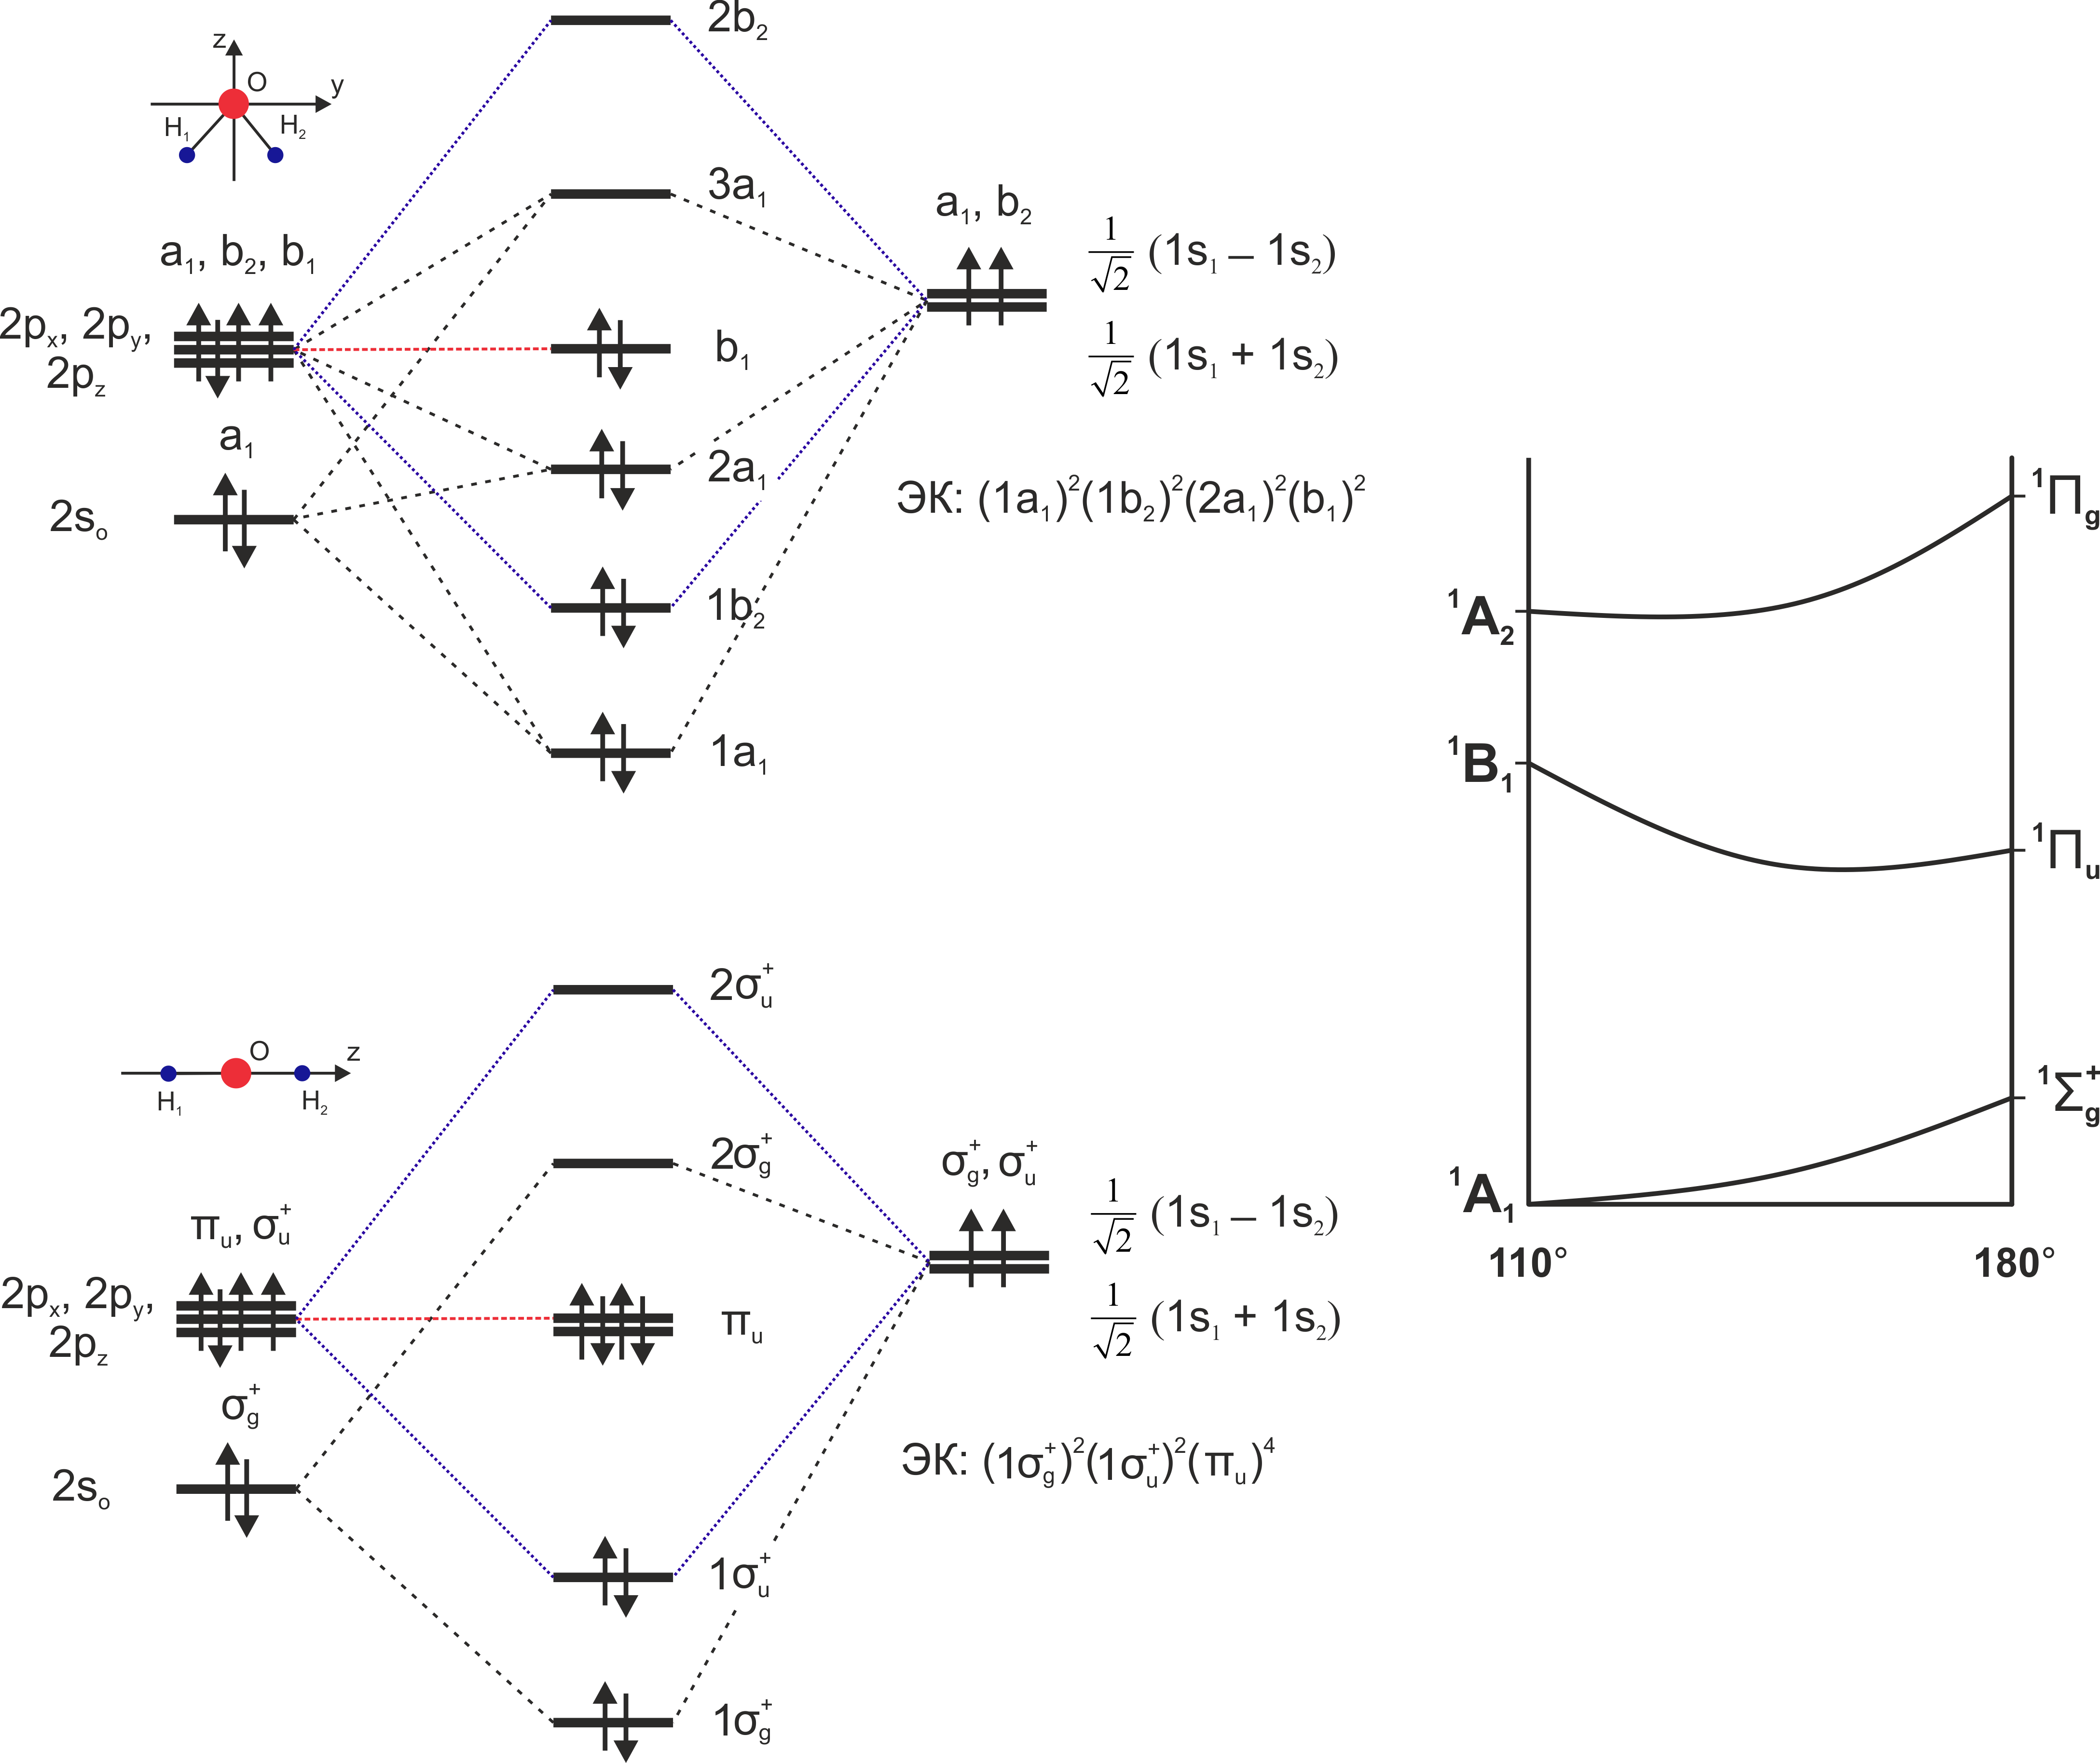
\includegraphics[width=9.4cm]{images/Fig_1_7_8_dec.png}
\centering
\end{figure}
\vspace{-\parskip}
\par
8. Задача 4 контрольной работы 2 осеннего семестра 2023/2024 учебного года. При учете интеграла перекрывания $S$ между соседними $p_z$ орбиталями для нахождения энергетических уровней и молекулярных орбиталей требуется решить следующее матричное уравнение:\par
\vspace{-\parskip}
\vspace{2mm}
\hspace{7mm}
$\begin{pmatrix}
\alpha-E & \beta-SE & 0 \\
\beta-SE & \alpha-E & \beta-SE \\
0 & \beta-SE & \alpha-E \\
\end{pmatrix}
\begin{pmatrix}
C_1 \\
C_2 \\
C_3 \\
\end{pmatrix}=0.$\par
\vspace{-\parskip}
\vspace{2mm}
Подставляя\hspace{\fill}$S=0,25$\hspace{\fill}получаем\hspace{\fill}энергии\hspace{\fill}$E_i$ равные\hspace{\fill}$\alpha$,\hspace{\fill}$1,55\alpha-2,19\beta$,\hspace{\fill}$0,74\alpha+1,04\beta$.\\ $E_{\Sigma}=2,48\alpha+2,08\beta$. Без учета $S$ энергетические уровни аллильного радикала: $\alpha$,~$\alpha-1,41\beta$, $\alpha+1,41\beta$, $E_{\Sigma}=3\alpha+2,82\beta$.\par
9. Образование молекулы ферроцена можно представить как взаимодействие катиона $\text{Fe}^{2+}$ ($3d^6$) и двух циклопентадиенильных анионов $\text{Cp}^-$. В качестве базиса орбиталей выберем $3d$ орбитали железа и $2p_z$ орбитали углерода, образующие ароматический цикл. Из-за высокой симметрии ферроцена ($D_{5d} / D_{5h}$) его можно рассматривать как квазилинейную систему в группе симметрии $D_{\infty h}$. В~этой группе $d$ орбитали железа будут иметь представления: $\Sigma_g^+$~($d_{z^2}$), $\Pi_g$~($d_{xz}, d_{yz}$), $\Delta_g$ ($d_{xy}, d_{x^2-y^2}$). Орбитали циклопентадиенила представляют собой две пятицентровые циклические системы, среди которых также найдутся комбинации с~симметрией $\Sigma_g^+$, $\Pi_g$ и $\Delta_g$. Для определенности можно считать, что взаимодействие $2p_z$ орбиталей между собой больше, чем с $d$ орбиталями железа. Итого 6~заполненных орбиталей двух Cp, далее расщепленные $d$ орбитали железа $\Delta_g$, $\Sigma_g^+$, $\Pi_g$ (в порядке увеличения энергии) и еще 4 незаполненные орбитали двух Cp. При переходе от группы $D_{\infty h}$ к $D_{5d}$ или $D_{5h}$ одномерное представление $\Sigma_g^+$  станет $А,$ двумерные $\Pi_g$ и $\Delta_g$ различными $Е$ представлениями. Таким образом качественно электронное строение можно описать конфигурацией для высокоспинового состояния Fe: $a^2(\text{Cp}) a^2(\text{Cp}) e^4(\text{Cp}) e^4(\text{Cp}) e^3(\text{Fe}) a^1(\text{Fe}) e^2(\text{Fe})$. Известно, что молекула ферроцена диамагнитна, поэтому более корректно будет рассматривать низкоспиное состояние комплекса: $a^2(\text{Cp}) a^2(\text{Cp}) e^4(\text{Cp}) e^4(\text{Cp}) e^4(\text{Fe}) a^2(\text{Fe})$. Оно соответствует полностью заполненной электронной конфигурации.\par
10. Задача 3 контрольной работы 2 осеннего семестра 2024/2025 учебного года. В данном ряду хюккелевских систем расположение энергетических уровней можно определить, например, используя теорию возмущений. Для каждого последующего $n$ происходит объединение двух одинаковых систем $n-1$, что дает поправки к энергиям $\pm \beta$. Кратность вырождения уровней при этом будет соответствовать биномиальным коэффициентам. Итого для произвольного $n$, обозначая $E_{\mu}=\alpha+\gamma_{\mu} \beta$, для заполненных МО получим для четных $n$ следующие величины кратности вырождения энергетического уровня и значения параметра $\gamma_{\mu}$:\par
\vspace{-\parskip}
\vspace{2mm}
\hspace{8mm}
\begin{tabular}{ |c|c|c|c|c| }
 КВ & $C_n^0$ & $C_n^1$ & $\ldots$ & $C_n^{n/2}$ \\ 
 $\gamma_{\mu}$ & $n$ & $n-2$ & $\ldots$ & $0$ \\  
\end{tabular}
\par
\vspace{-\parskip}
\vspace{3mm}
Для нечетных $n$:
\par
\vspace{-\parskip}
\vspace{2mm}
\hspace{8mm}
\begin{tabular}{ |c|c|c|c|c| }
 КВ & $C_n^0$ & $C_n^1$ & $\ldots$ & $C_n^{(n-1)/2}$ \\ 
 $\gamma_{\mu}$ & $n$ & $n-2$ & $\ldots$ & $1$ \\  
\end{tabular}\par
\vspace{-\parskip}
\vspace{2mm}
Свободные МО расположены симметрично, так как все рассматриваемые системы с $n > 1$ являются четными альтернантными. Полная электронная энергия определяется соответствующей суммой. Случай четного $n$:
\begin{equation*}
\begin{aligned}
& E_{\Sigma}=2^n \alpha+2\sum_{i=0}^{n/2} C_n^i (n-2i)\beta = \ldots = 2^n \alpha + (2+n)\beta C_n^{(n+2)/2}.\hspace{13mm}
\end{aligned}
\end{equation*}
Для нечетного $n$ аналогично:
\begin{equation*}
\begin{aligned}
& E_{\Sigma}= 2^n \alpha + 2\beta n C_{n-1}^{(n-1)/2} = 2^n \alpha + (1+n) \beta C_{n}^{(n+1)/2}.\hspace{27mm}
\end{aligned}
\end{equation*}
\par
\vspace{-\parskip}
%\hspace{\fill}
11. Группа симметрии молекулы $D_{3h}$. Симметрия и энергия молекулярных орбиталей: $1a_{2}''$ $E_1=\alpha+\sqrt6\beta$, $1e''$ $E_{2,3}=\alpha+\sqrt3 \beta$, $2a_{2}''$ $E_4=\alpha+\beta$, $2e''$ $E_{5,6}=\alpha+\beta$, $a_{1}''$~$E_7=\alpha$, $3a_{2}''$ $E_8=\alpha-\beta$, $3e''$ $E_{9,10}=\alpha-\beta$, $4e''$ $E_{11,12}=\alpha-\sqrt3 \beta$, $4a_{2}''$ $E_{13}=\alpha-\sqrt6 \beta$. По~теории возмущений данную молекулу можно рассматривать как циклическую систему из 12 центров и дополнительный атом в середине, что приводит к~вырожденной теории возмущений для уровней $E=\alpha$. Итоговые энергии и симметрии в первом порядке теории возмущений: $1a_{2}''$ $E_1=\alpha+2\beta$, $1e''$~$E_{2,3}=\alpha+\sqrt3 \beta$, $2a_{2}''$ $E_4=\alpha+\sqrt{3/2} \beta$, $2e''$ $E_{5,6}=\alpha+\beta$, $a_{1}''$ $E_7=\alpha$, $3e''$ $E_{8,9}=\alpha-\beta$, $3a_{2}''$ $E_{10}=\alpha-\sqrt{3/2} \beta$, $4e''$ $E_{11,12}=\alpha-\sqrt3 \beta$, $4a_{2}''$ $E_{13}=\alpha-2 \beta$. Во втором порядке теории возмущений поправка к энергии будет только для уровней с симметрией $a_2''$~с~энергией $E = \alpha \pm 2\beta$. Она равна $\Delta E^{(2)}= |\braket{\psi(a_2'')|V|\psi_{13}}|^2/(\pm 2\beta) = \pm 3/8 \beta$. Итоговые энергии МО:~$1a_{2}''$ $E_1=\alpha+2,375\beta$, $1e''$ $E_{2,3}=\alpha+\sqrt3 \beta$, $2a_{2}''$ $E_4=\alpha+\sqrt{3/2} \beta$, $2e''$ $E_{5,6}=\alpha+\beta$, $a_{1}''$~$E_7=\alpha$, $3e''$ $E_{8,9}=\alpha-\beta$, $3a_{2}''$ $E_{10}=\alpha-\sqrt{3/2} \beta$, $4e''$ $E_{11,12}=\alpha-\sqrt3 \beta$, $4a_{2}''$ $E_{13}=\alpha-2,375 \beta$.\par
12. Задача 3 контрольной работы 2 осеннего семестра 2023/2024 учебного года. Самая коротковолновая линия поглощения $\pi$-системы пентадиенильного радикала соответствует переходу между молекулярными орбиталями с~минимальной и максимальной энергией. В группе симметрии $C_{2v}$ данные орбитали соответствуют $B_2$~неприводивому представлению. Таким образом, указанный переход соответствует $\pi$~поляризации.\par
13. Задача 1 контрольной работы 2 осеннего семестра 2022/2023 учебного года. Группа симметрии молекулы $D_{2h}$. Симметрия и энергия молекулярных орбиталей: $1b_{1u}$ $E_1=\alpha+2,34\beta$, $1b_{2g}$ $E_2=\alpha+1,81\beta$, $2b_{1u}$ $E_3=\alpha+0,47\beta$, $a_{u}$ $E_4=\alpha$, $b_{3g}$~$E_5=\alpha$, $2b_{2g}$ $E_6=\alpha-0,47\beta$, $3b_{1u}$ $E_7=\alpha-1,81\beta$, $3b_{2g}$ $E_8=\alpha-2,34\beta$. Электронная конфигурация основного состояния $(1b_{1u})^2 (1b_{2g})^2 (2b_{1u})^2 (a_u)^1 (b_{3g})^1$. Основной терм $^3B_{3u}$.\par
\newpage

\subsection{Специальные хюккелевские системы}
1. Электронная конфигурация циклобутадиена $(a_{2u})^2(e_g)^2$ , если считать, что его $\pi$-система относится к группе симметрии $D_{4h}$ (ось $x$ направлена вправо между атомами углерода, ось $y$ направлена вверх между атомами углерода). Основной терм $^3A_{2g}$.\par
2. Все МО орбитали в линейной хюккелевской системе невырождены, поэтому данная система будет являться радикалом только при $n=4k+1$ и $n=4k+3$, где $k=0,1,2,\ldots$. Пусть система относится к группе симметрии $D_{\infty h}$, симметрии МО чередуются и общее количество разрешенных переходов: (1) $N=\frac{(n-1)(n+3)}{8}$, если $n=4k+1$; (2) $N=\frac{(n+1)(n+1)}{8}$, если $n=4k+3$. Число разрешенных переходов с различной энергией равно $N_{\text{E}}=N/2$, если $n = 4k+1,\,4k+3$, так как энергетические уровни расположены симметрично относительно уровня $E=\alpha$.\par
3. Используя вырожденную теорию возмущений для учета индуктивного заместителя с помощью единственного ненулевого матричного элемента оператора возмущения: $\bra{\phi_1} V \ket{\phi_1}=\xi \beta$, $\xi<0$, можно определить, что $E_{\text{ВЗМО}}=\alpha$, если $n=4k$ и $E_{\text{ВЗМО}}=\alpha+2\beta \sin{\frac{\pi}{n}}+\frac{2}{n}\xi \beta$, если $n=4k+2$.\par
4. Задача 5 дифференциального зачета осеннего семестра 2022/2023 учебного года. Описанная ситуация соответствует переходу между термами $^2B_{2g} \rightarrow\,\,^2B_{1u}$, который разрешен в $\sigma$ поляризации.\par
5. Согласно методу Хюккеля у бесконечного сопряженного полиена можно было бы ожидать появления металлической проводимости, так как энергетический зазор между заполненными и свободными молекулярными орбиталями в~такой системе должен быть близок к нулю. Расстояние между энергетическими уровнями с максимальной и минимальной энергией $\Delta E \rightarrow 4\beta$, если $n \rightarrow \infty$.  \par
6. Данная система является нечетной альтернантной. Исходя из орбитали неспаренного электрона можно определить ненулевые спиновые плотности на различных центрах: $\rho_1 = 25/56$, $\rho_2 = 7/32$, $\rho_{3,\,4,\,5,\,9,\,12} = 9/224$, $\rho_6 = 1/14$, $\rho_{7,\,10} = 1/224$,  $\rho_{8,\,11,\,13} = 1/56$. Для расчета спиновой плотности меченые центры пронумерованы в порядке сверху вниз, слева направо.\par
7. Используя общее решение для циклических систем можно определить, что порядок связи, например, между центрами 1 и $n$, равен $b_{1n}=\frac{2}{n}\sin^{-1}{\frac{\pi}{n}}$.\par
8. Формально нельзя, так как несмотря на различную симметрию, в обоих случаях в спектре поглощения будет 1 линия с энергией $2\beta$. При этом для квадратной геометрии основной триплетный терм $^3A_{2g}$ и синглетные термы $^1A_{1g}$, $^1B_{1g}$, $^1B_{2g}$, соответствующие этой же электронной конфигурации $(a_{2u})^2(e_g)^2$, имеют близкую, но неодинаковую энергию энергию, что может привести к~большему количеству линий в спектре поглощения, в сравнении с прямоугольной геометрией и соответствующей ей полностью заполененной электронной конфигурацией.\par
9. Случай $\text{H}_3^+$. Полная электронная энергия $E_{\Sigma}$: (1), (2) $2\alpha + 2\sqrt2 \beta$; (3) $2\alpha + 4 \beta$. Спиновая плотность $\rho_i$ равна 0 на всех центрах для всех структур. Порядок связи $b_{ij}$: (1), (2) $b_{12}=b_{23}=\sqrt2 / 2$, $b_{13}=1/2$; (3) $b_{12}=b_{23}=b_{13}=2/3$. Наиболее выгодной является циклическая структура.\\
Случай $\text{H}_3$. Полная электронная энергия $E_{\Sigma}$: (1), (2) $3\alpha + 2\sqrt2 \beta$; (3) $3\alpha + 3 \beta$. Спиновая плотность $\rho_i$: (1), (2) $\rho_{1,\,3}=1/2$, $\rho_2=0$; (3) $\rho_{1,\,2,\,3}=1/3$. Порядок связи $b_{ij}$: (1),~(2)~$b_{12}=b_{23}=\sqrt2 / 2$, $b_{13}=0$; (3) $b_{12}=b_{23}=b_{13}=1/2$. Наиболее выгодной является циклическая структура.\\
Случай $\text{H}_3^-$. Полная электронная энергия $E_{\Sigma}$: (1), (2) $4\alpha + 2\sqrt2 \beta$; (3) $4\alpha + 2 \beta$. Спиновая плотность $\rho_i$: (1), (2) 0 на всех центрах; (3) $\rho_{1,\,2,\,3}=2/3$.  Порядок связи $b_{ij}$: (1),~(2)~$b_{12}=b_{23}=\sqrt2 / 2$, $b_{13}=-1/2$; (3) $b_{12}=b_{23}=b_{13}=1/3$. Наиболее выгодной является угловая и линейная структура, которые в рамках метода Хюккеля не~отличаются.\par
10. Задача 4 контрольной работы 2 осеннего семестра 2022/2023 учебного года. Для полносвязанной системы с $n$ центрами будет однократно вырожденный уровень с $E = \alpha + (n - 1)\beta$ и $(n - 1)$-кратно вырожденный уровень с энергией $E = \alpha - \beta$. Полная электронная энергия $E_{\Sigma} = n(\alpha + \beta)$.\par
11. В обоих случаях данная система является нечетной альтернантной системой. При этом количество меченых и немеченых центров отличается на 2, то есть это дирадикал. Определяя по две орбитали неспаренного электронного для каждого случая можно посчитать ненулевые спиновые плотности на различных центрах: (1) $\rho_{1,\,2,\,3,\,4} = 1/2$, (2) $\rho_{2,\,3,\,4,\,5} = 1/2$. Меченые центры пронумерованы в порядке сверху вниз, слева направо.\par
\newpage

\subsection{Применение теории возмущений}
1. Задача 1 контрольной работы 2 осеннего семестра 2021/2022 учебного года. В~рамках теории возмущений первого порядка волновые функции не меняются. Порядок связи останется таким же, как в невозмущенном этилене $b_{12}=1$. Во втором порядке теории возмущений при учете заместителя с помощью возмущения $\bra{\phi_1} V \ket{\phi_1}=\xi \beta$ порядок связи станет равным $b_{12}'=\frac{16-\xi ^2}{16+ \xi ^2}$.\par
2. Разделим $\pi$-систему нафталина на две одинаковых линейных $\pi$-системы из 5 центров. Центры в этих линейных системах пронумерованы по порядку $\phi_1 - \phi_5$ и $\phi_1' - \phi_5'$, соответственно. Образование нафталина из них соответствует возмущению $\bra{\phi_1}V \ket{\phi_1'}=\bra{\phi_3} V \ket{\phi_3'}=\bra{\phi_5} V \ket{\phi_5'}=\beta$. Применяя теорию возмущений для вырожденного случая к нижним МО линейных систем можно найти поправки к их энергии $\Delta E_{1,2}= \pm \beta/2 $. Минимальная энергия соответствует поправке равной $\Delta E_1 = \beta/2$ с правильной волновой функцией $\psi=\frac{1}{\sqrt{24}}(\phi_1+\sqrt3\phi_2+2\phi_3+\sqrt3\phi_4+\phi_5+\phi_1'+\sqrt3\phi_2'+2\phi_3'+\sqrt3\phi_4'+\phi_5')$. Энергия данной орбитали $E\approx \alpha+2,33\beta$. \par
3. Изменение длин связей изменяет резонансный интеграл между соответствующими центрами. Введем возмущение $\bra{\phi_1} V \ket{\phi_2}=\bra{\phi_3} V \ket{\phi_4} = -0,1\beta$, что соответствует увеличению длин связи между центрами 1-2 и 3-4, соотвественно. После применения теории возмущений к заполненным уровням циклической системы получим: $E_{1}= \alpha+1,9\beta$, $E_{2,3}=\alpha\pm 0,1\beta$. Итого $E_{\Sigma}=4\alpha+4\beta$, то~есть $\Delta E_{\Sigma}=0$. В случае уменьшения длин связей возмущение будет иметь вид $\bra{\phi_1}V\ket{\phi_2}=\bra{\phi_3}V\ket{\phi_4}=0,1\beta$. Аналогичные вычисления дают $\Delta E_{\Sigma}=0,2\beta$.\par
\begin{wrapfigure}{r}{47mm} %this figure will be at the right
    \centering
    \vspace{0mm}
    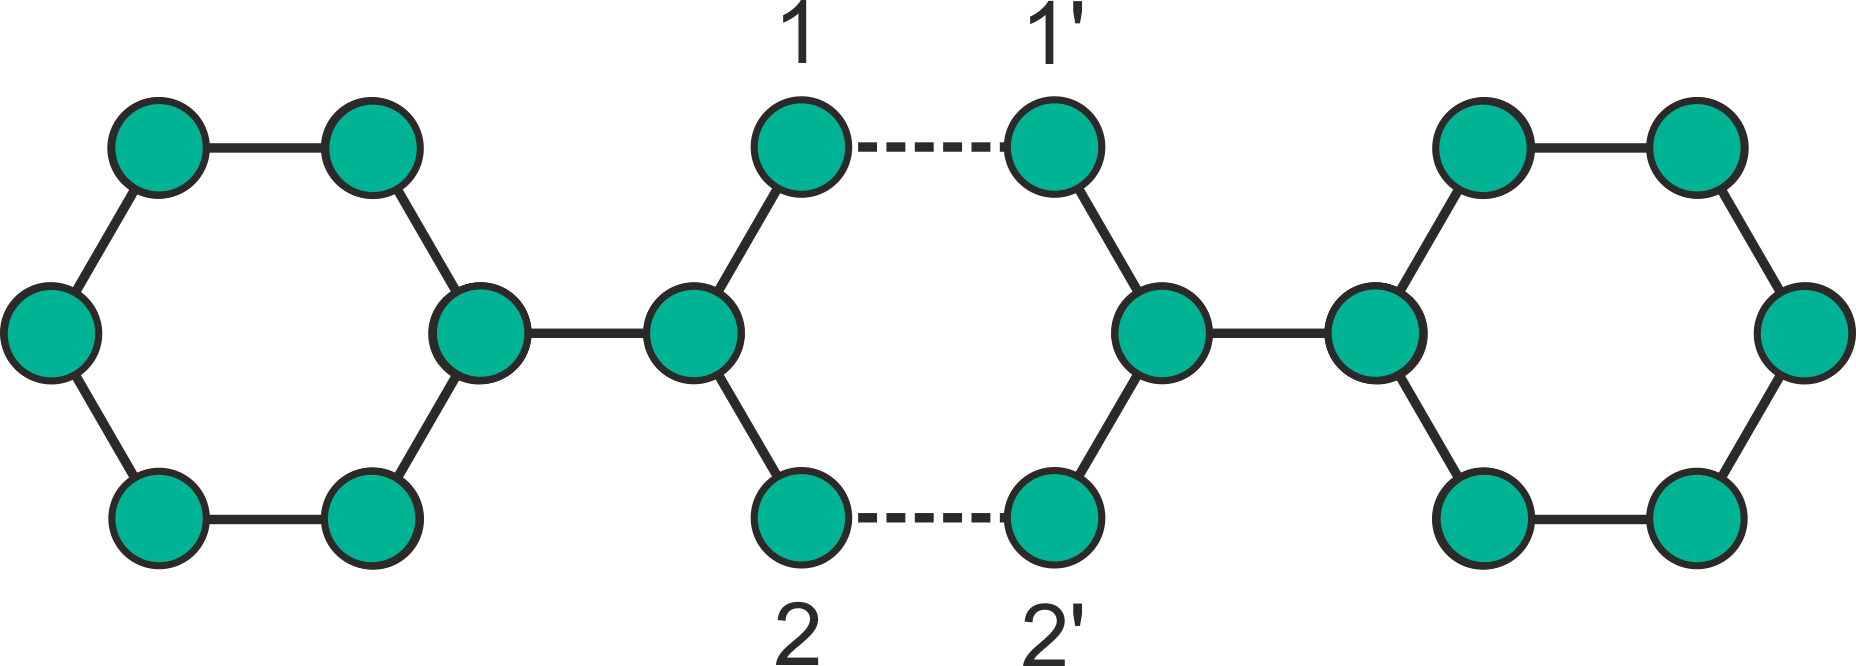
\includegraphics[width=40mm]{images/Fig_1_9_4_dec.png}
    \vspace{-5mm}
\end{wrapfigure}
4. Разделим $\pi$-систему п-терфенила на две одинаковых альтернантных системы, как показано на рисунке справа. Молекулярные орбитали неспаренного электрона: $\psi_{\textrm{НЭ}_1}=\frac{1}{\sqrt2}(\phi_1 -\phi_2)$ и $\psi_{\textrm{НЭ}_2}=\frac{1}{\sqrt2}(\phi_1' -\phi_2')$. Данные уровни вырождены, имеют энергию $E_{1,2}=\alpha$ и на них расположено 3 электрона (анион-радикал). Возмущение вида $\bra{\phi_1}V\ket{\phi_1’}=\bra{\phi_2}V\ket{\phi_2’}=\beta$ приводит к~поправкам к энергии $\Delta E_{1,2}=\pm \beta$. Тогда неспаренный электрон будет локализован на уровне, соответствующем поправке $\Delta E =-\beta$. Его правильная волновая функция имеет вид $\psi_{\textrm{НЭ}}=\frac{1}{\sqrt{2}}(\psi_{\textrm{НЭ}_1}-\psi_{\textrm{НЭ}_2})=\frac{1}{2}(\phi_1 -\phi_2-\phi_1' +\phi_2')$. Итого спиновая плотность равна $\rho_{1,\,2,\,1',\,2'}=1/4$.\par
5. Задача 5 контрольной работы 2 осеннего семестра 2023/2024 учебного года. Промежуточное состояние во всех случаях является одинаковой нечетной альтернантной системой. Используя МО неспаренного электрона можно посчитать $\pi$-заряд на центрах I, II, III: $q_{\text {I}}=26/51$; $q_{{\text {II}}}=1;$ $ q_{{\text {III}}}=50/51$. Тогда в~первом порядке теории возмущений изменение полной электронной энергии при введении –CH$_3$ группы в положение I, II или III: $\Delta E_{\text {I}}=26/51 \xi \beta$; $\Delta E_{{\text {II}}}=\xi \beta$; $\Delta E_{{\text {III}}}=50/51 \xi \beta$. Таким образом, повышение энергетического барьера меньше при замещении по положению I.\par
6. Вводим индуктивные заместители в $\pi$-систему бензола по теории возмущений: $\bra{\phi_1}{V}\ket{\phi_1}=\bra{\phi_2}{V}\ket{\phi_2}=\bra{\phi_4}{V}\ket{\phi_4}=\bra{\phi_5}{V}\ket{\phi_5}=\xi\beta$, где $ \xi=-0,1$. Поправки к энергиям уровней $E_{2,3}$ и $E_{4,5}$ равны $\Delta E_2 =\Delta E_4=\frac{1}{3}\xi\beta$, $\Delta E_3=\Delta E_5=\xi\beta$. Волновые функции не изменяются. В анион-радикале МО неспаренного электрона $\psi_4=\frac{1}{\sqrt{12}}(\phi_1+\phi_2-2\phi_3+\phi_4+\phi_5-2\phi_6)$, $\rho_{1,\,2,\,4,\,5}=1/12, \rho_{3,\,6}=1/3$. В~катион-радикале МО неспаренного электрона $\psi_3=\frac{1}{2}(\phi_1+\phi_2-\phi_4-\phi_5)$, $\rho_{1,\,2,\,4,\,5}=1/4$. Самый длинноволновый электрический дипольный переход имеет наименьшую энергию. В бензоле ($D_{6h}$) это переход из электронной конфигурации $(a_{2u})^2(e_{1g})^4$ терм $^1A_{1g}$ в конфигурацию $(a_{2u})^2(e_{1g})^3(e_{2u})^1$ термы $^{3,1}B_{1u}, {^{3,1}B_{2u}}, {^{3,1}E_{1u}}$. Переход $^1A_{1g}$ $\rightarrow$ ${^{1}E_{1u}}$ разрешен в $\sigma$ поляризации, Энергия перехода равна $\Delta E =-2\beta$. Cимметрия дурола $D_{2h}$. Наиболее длиноволновый переход имеет энергию $\Delta E \approx -1,933\beta$ и соответствует переходу с $\psi_3$ на $\psi_4$. Это переход из электронной конфигурации $(b_{1u})^2(b_{2g})^2(b_{3g})^2$ терм $^1{A_{g}}$ в конфигурацию $(b_{1u})^2(b_{2g})^2(b_{3g})^1(b_{1u})^1$ термы $^{3,1}{B_{2u}}$. Переход $^{1}{A_{g}}$ $\rightarrow$ $^{1}{B_{2u}}$ разрешен в $\sigma$ поляризации.\par
7. Для сравнения относительной устойчивости $\pi$-систем антрацена и фенантрена каждую из них удобно разделить на две одинаковые линейные альтернантные системы из 7 центров. Объединяя их назад по теории возмущений можно показать, что $\pi$-система антрацена является более устойчивой: $\Delta E_{\textrm{А}}=2\beta$; $\Delta E_{\textrm{Ф}}=3\beta / 2$.\par
8. Промежуточное состояние в данной реакции представляет собой $\pi$-систему аллильного радикала с дополнительным электроном ($S_N Ar$). В промежуточном состоянии $\pi$-заряд на центрах равен $q_{1,\,3}=3/2$, $q_{2}=1$. Используя выражение для изменения полной электронной энергии при введении заместителя $\Delta E^{(1)}=\sum_j q_j\Delta\alpha_j$, где $q_j$ – $\pi$-заряд на центре $j$, $\Delta\alpha_j$ – изменение кулоновского интеграла для $j$-того центра, можно показать, что нуклеофильное ароматическое замещение преимущественно реализуется в положение, расположенное ближе к –CF$_3$ группе, $\Delta E^{(1)}=0,35\beta$.\par
9. Задача 3 контрольной работы 2 осеннего семестра 2022/2023 учебного года.  Промежуточное состояние в обоих случаях является одинаковой нечетной альтернантной системой. Используя МО неспаренного электрона и $\pi$-заряд, в первом порядке теории возмущений определяем изменение полной электронной энергии при введении –CH$_3$ группы в положение 1 или 2: $\Delta E_1=3/2 \xi \beta$; $\Delta E_2=\xi \beta$. Таким образом, повышение энергетического барьера меньше при~замещении по положению 2.\par
10. Промежуточное состояние в данной реакции представляет собой альтернантную систему пентадиенильного радикала с 4 ($S_E Ar$) или 6 ($S_N Ar$) электронами. В случае нуклеофильного ароматического замещения $\pi$-заряд равен $q_{1,\,3,\,5}=4/3$, $q_{2,\,4}=1$. В случае электрофильного ароматического замещения $\pi$-заряд равен $q_{1,\,3,\,5}=2/3$, $q_{2,\,4}=1$. Используя теорию возмущений можно показать, что нуклеофильное замещение преимущественно протекает в положение 3, расположенное ближе к –CF$_3$ группе, $\Delta E^{(1)} = 0,3\beta$. Аналогично, электрофильное замещение преимущественно протекает в положение 2, расположенное ближе к –CH$_3$ группе, $\Delta E^{(1)}\approx 0,233\beta$.\par
\begin{wrapfigure}{r}{20mm} %this figure will be at the right
    \centering
    \vspace{-2ex}
    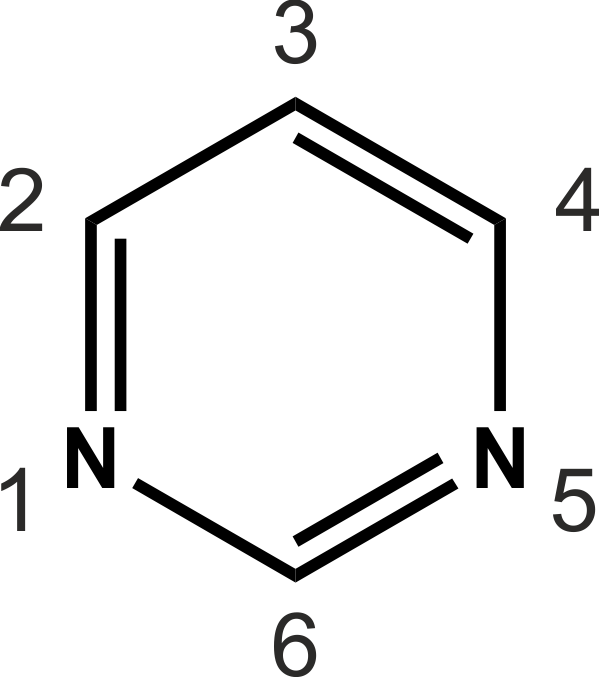
\includegraphics[width=12mm]{images/Fig_1_9_11_dec.png}
    \vspace{-5mm}
\end{wrapfigure}
11. Теоретический вопрос 2 дифференциального зачета осеннего семестра 2024/2025 учебного года. Изменяя кулоновский интеграл атома углерода на кулоновский интеграл атома азота по теории возмущений и нумеруя центры в пиримидине так, как показано на рисунке, можно получить МО неспаренного электрона: $\psi_{\text{НЭ}}=\frac{1}{\sqrt{12}}(2\phi_6+\phi_1+\phi_5-2\phi_3-\phi_2-\phi_4)$. Таким образом, спиновая плотность равна $\rho_{1,\,2,\,4,\,5}=1/12$; $\rho_{3,\,6}=4/12$.\par
\begin{wrapfigure}{r}{20mm} %this figure will be at the right
    \centering
    \vspace{-2ex}
    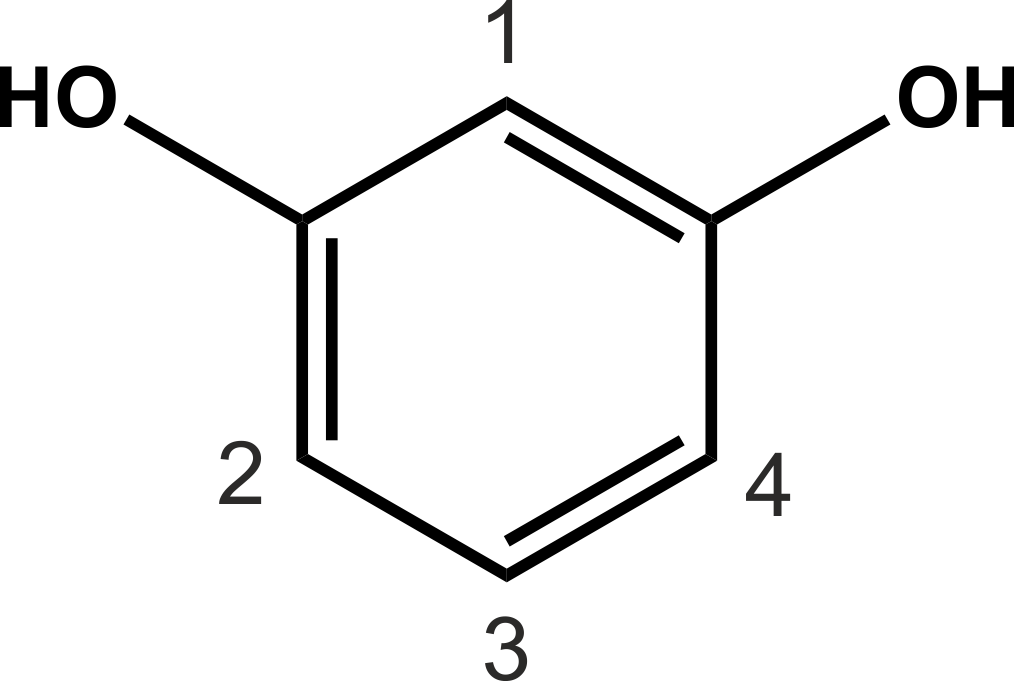
\includegraphics[width=19mm]{images/Fig_1_9_12_dec.png}
    \vspace{0mm}
\end{wrapfigure}
12. Группа –OH является +M мезомерным заместителем. Для определения преимущественного направления электрофильного замещения необходимо использовать второй порядок теории возмущений. Поправка к полной электронной энергии для случая электрофильного замещения при введении +M~заместителя может быть определена по выражению:
\begin{equation*}
\begin{aligned}
& \Delta E_{\Sigma}^{(2)}=2\sum_{\mu = m+1}^{n} \frac{C_{\mu r}^2 k^2}{h-\gamma_{\mu}} \beta, \hspace{58mm}
\end{aligned}
\end{equation*}
где $\alpha_{\text{O}}=\alpha_{\text{C}}+h\beta$, $\bra{\phi_{\text{O}}} V \ket{\phi_{\text{C}}}=k\beta$, $r$ – номер центра с –OH группой, $m$ – порядковый номер ВЗМО промежуточного состояния, $C_{\mu r}$ – коэффициент перед $r$-тым центром в $\mu$-той МО промежуточного состояния, $n$ – количество МО в~промежуточном состоянии. В данной задаче промежуточное состояние представляет собой $\pi$-систему пентадиенильного радикала с 4 электронами. Тогда, обозначая различные положения замещения как показано на рисунке, а также используя $h=1,2$ и $k=1,1$ получаются следующие поправки: (1) Положение 1: $2,032\beta$, (2) Положения 2, 4: $1,963\beta$, (3) Положение 3: $0,963\beta$. Таким образом, положение 1 является преимущественным направлением электрофильного замещения в~молекуле резорцина.\par
13. Необходимо сравнить полную электронную энергию $\pi$-систем промежуточных состояний, возникающих в процессе протекания данной реакции. Возможные варианты: (1) Замещение в положения 1, 2; Остается $\pi$-система бутадиена, $E_{\Sigma}\approx 4\alpha+4,47\beta$; (2) Замещение в положения 1, 3; Остается $\pi$-система аллильного радикала и изолированный центр, $E_{\Sigma}= 4\alpha+2\sqrt2\beta$; (3) Замещение в~положения 1, 4; Остаются две изолированных $\pi$-системы этилена, $E_{\Sigma}= 4\alpha+4\beta$. Полная электронная энергия минимальна в случае (1), который и является преимущественным направлением замещения. Полная электронная энергия промежуточного состояния для случая (2) отличается от случая (1) незначительно. Разница между данными вариантами может быть компенсирована характеристиками присоединяющихся радикальных частиц, например стерическим фактором. Наименее выгодным вариантом является вариант (2).\par
14. В бензоле ($D_{6h}$) самой высокой энергии соответствует запрещенный переход между конфигурациями $(a_{2u})^2(e_{1g})^4$ терм $^1{A_{1g}}$ и $(a_{2u})^1(e_{1g})^4(b_{2g})^1$ термы $^{3,1}B_{1u}$. Атомы дейтерия отличаются от атомов водорода кулоновским интегралом, который меняется на величину $\Delta \alpha =\alpha\frac{m_e}{2m_H} < 0$, см. задачу 1.2. Далее используем первый порядок теории возмущений: (1) $\bra{\phi_3}V\ket{\phi_3}=\bra{\phi_4}V\ket{\phi_4}=\Delta \alpha$ в случае 1,2-дидейтеробензола, (2)~$\bra{\phi_3}V\ket{\phi_3}=\bra{\phi_5}V\ket{\phi_5}=\Delta \alpha$ для 1,3-дидейтеробензола, (3)~$\bra{\phi_3}V\ket{\phi_3}=\bra{\phi_6}V\ket{\phi_6}=\Delta \alpha $ для 1,4-дидейтеробензола. Во всех случаях возмущение приводит к поправке $\Delta E_{1,\,6}^{(1)}= \Delta \alpha/3 $. Энергия перехода не~изменится и~различить изомеры не получится. При этом в отличие от бензола молекулы дидейтеробензола обладают более низкой симметрией, из-за чего для всех изомеров данный переход становится разрешенным.\par
15. Задача 2 дифференциального зачета осеннего семестра 2023/2024 учебного года. Направление преимущественного присоединения можно определить сравнивая индекс локализации для указанных трех случаев протекания реакции: $L=\sum_{\mu} n_{\mu}  \gamma_{\mu}^{\text{нач}} - \sum_{\mu} n_{\mu}  \gamma_{\mu}^{\text{кон}}$, где $n_{\mu}$ – количество электронов на $\mu$-ой МО, $\gamma_{\mu}$ – коэффициенты перед резонансными интегралами в энегрии $\mu$-ой МО: $\varepsilon_{\mu}=\alpha+\gamma_{\mu} \beta$. Поскольку начальное состояние во всех трех случаях одинаковое, то достаточно проанализировать второе слагаемое: $L'=\sum_{\mu} n_{\mu}  \gamma_{\mu}^{\text{кон}}$. Чем оно больше, тем вероятнее реакция. Центр I: конечное состояние – две $\pi$-системы этилена, $L'=4$; Центр II: конечное состояние – $\pi$-система аллильного радикала и изолированный центр, $L'=2,82$; Центр III: конечное состояние – $\pi$-система бутадиена, $L'=4,48$. Центр III является преимущественным направлением реакции присоединения атома водорода.\par
\newpage

%\usepackage[fit, breakall]{truncate}
%\phantomsection
\section[Спектроскопические методы исследования вещества]{\texorpdfstring{Электронное строение координационных соединений.\\Спектроскопические методы исследования вещества}{Электронное строение координационных соединений. Спектроскопические методы исследования вещества}}
%\addcontentsline{toc}{chapter}{2 Электронное строение координационных соединений. Спектроскопические методы исследования }
%\markboth{Электронное строение координационных соединений. Спектроскопические методы исследования}{Электронное строение координационных соединений. Спектроскопические методы исследования}
\subsection{Правила Вудворда-Хоффмана}
\begin{wrapfigure}{r}{30mm} %this figure will be at the right
    \centering
    \vspace{1.8mm}
    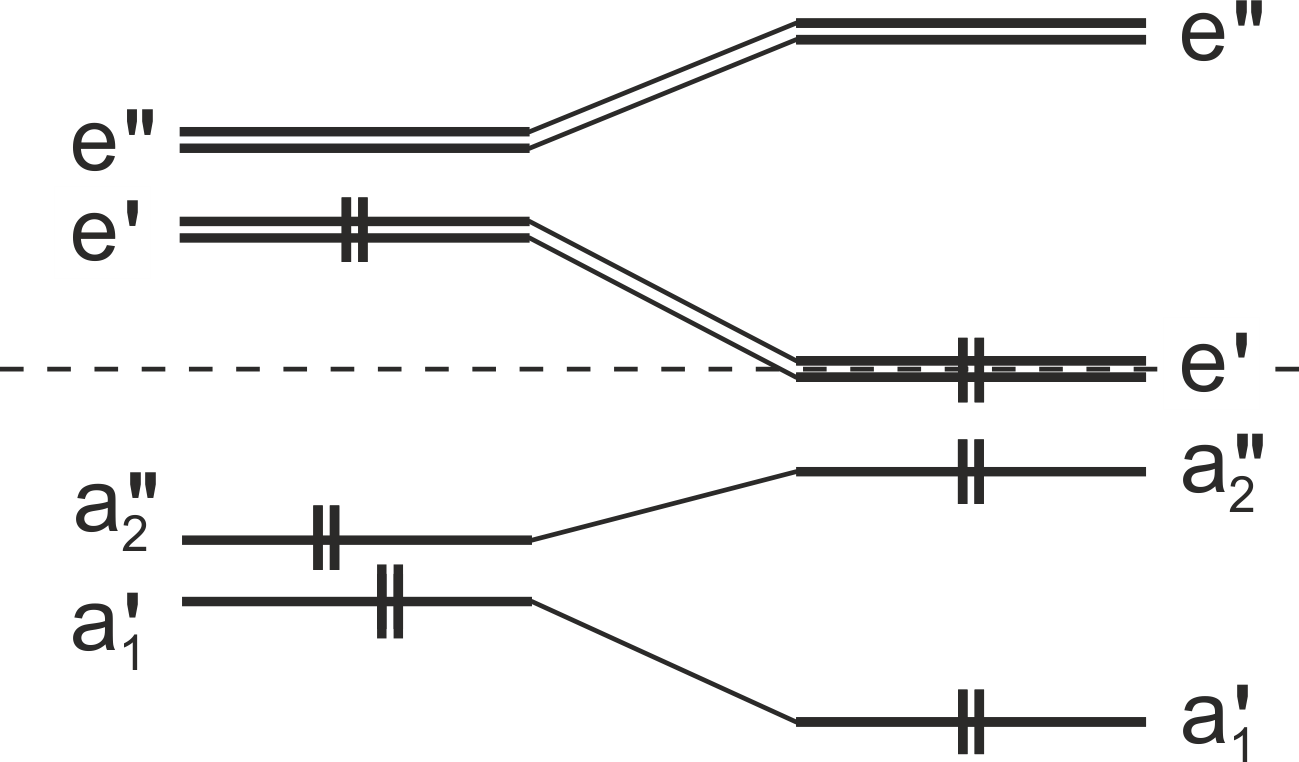
\includegraphics[width=30mm]{images/Fig_2_1_1_dec.png}
    \vspace{-5mm}
\end{wrapfigure}
1. Задача 3 контрольной работы 1 весеннего семестра 2021/2022 учебного года. Корреляционная диаграмма для группы симметрии $D_{3h}$ приведена на рисунке ниже.  Считая, что в реагентах молекулярные орбитали с симметрией $a'_1$ и $a''_2$, а также орбитали $e'$ и $e''$ имеют одинаковую энергию, изменение полной электронной энергии равно $2\beta$. Реакция разрешена термически.\par
\begin{wrapfigure}{r}{30mm} %this figure will be at the right
    \centering
    \vspace{-2.2mm}
    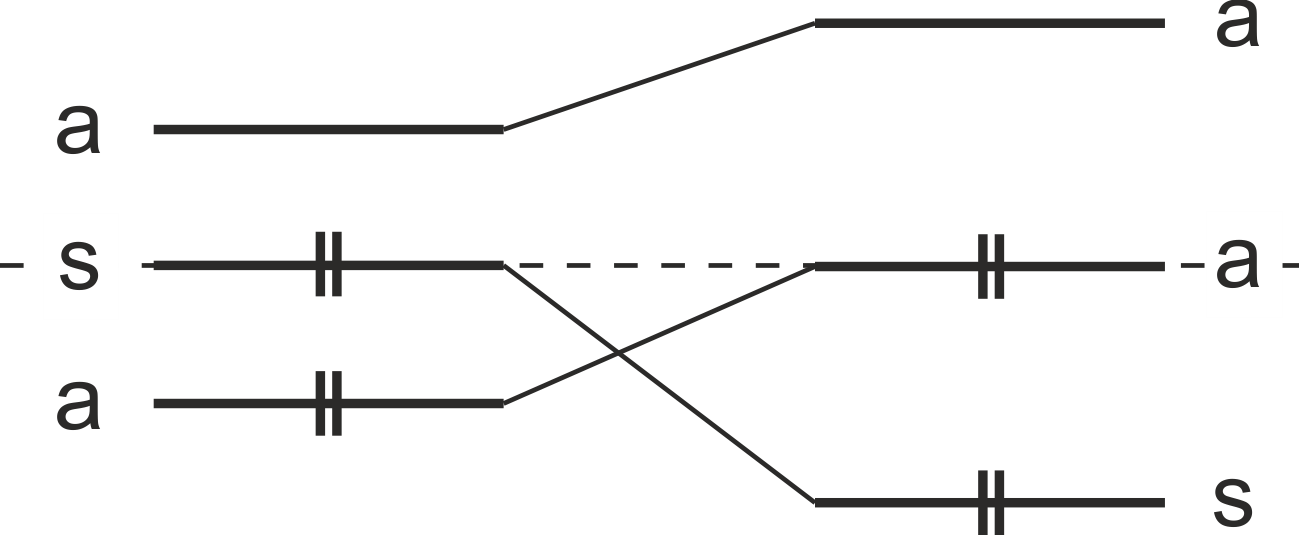
\includegraphics[width=30mm]{images/Fig_2_1_2_dec.png}
    \vspace{-5mm}
\end{wrapfigure}
2. Задача 1 контрольной работы 1 весеннего семестра 2023/2024 учебного года. Данная реакция термически протекает в конротаторном механизме, поэтому продуктом является цис-изомер, соответствующая корреляционная диаграмма приведена на рисунке.\par
3. В ходе реакции сохраняется группа симметрии $C_2$, при этом меняется направление единственной оси симметрии данной группы. Аналогично можно рассмотреть группу симметрии $D_2$. Реакция запрещена термически. Связывающая молекулярная орбиталь (МО) реагентов симметрии $b$ в базисе $2p_z$ атомных орбиталей становится разрыхляющей орбиталью продуктов, разрыхляющая МО реагентов симметрии $a$ становится связывающей орбиталью продуктов.\par
4. В $4\pi_s$ + $2\pi_s$ топологии реакция разрешена термически, есть ровно один $4n+2$ супра-компонент. В супра-/антара- топологии реакция запрещена термически, так как она соответствует, например, $2\pi_s$ + $2\pi_s$ + $2\pi_a$ компонентам. Корреляционная диаграмма для супра-/супра- топологии приведена на~рисунке. Для случая супра-/антара- топологии корреляционную диаграмму построить нельзя. В ходе реакции не сохраняется ни один элемент симметрии, см. рисунок.\par
\vspace{-\parskip}
\vspace{1mm}
\begin{figure}[h]
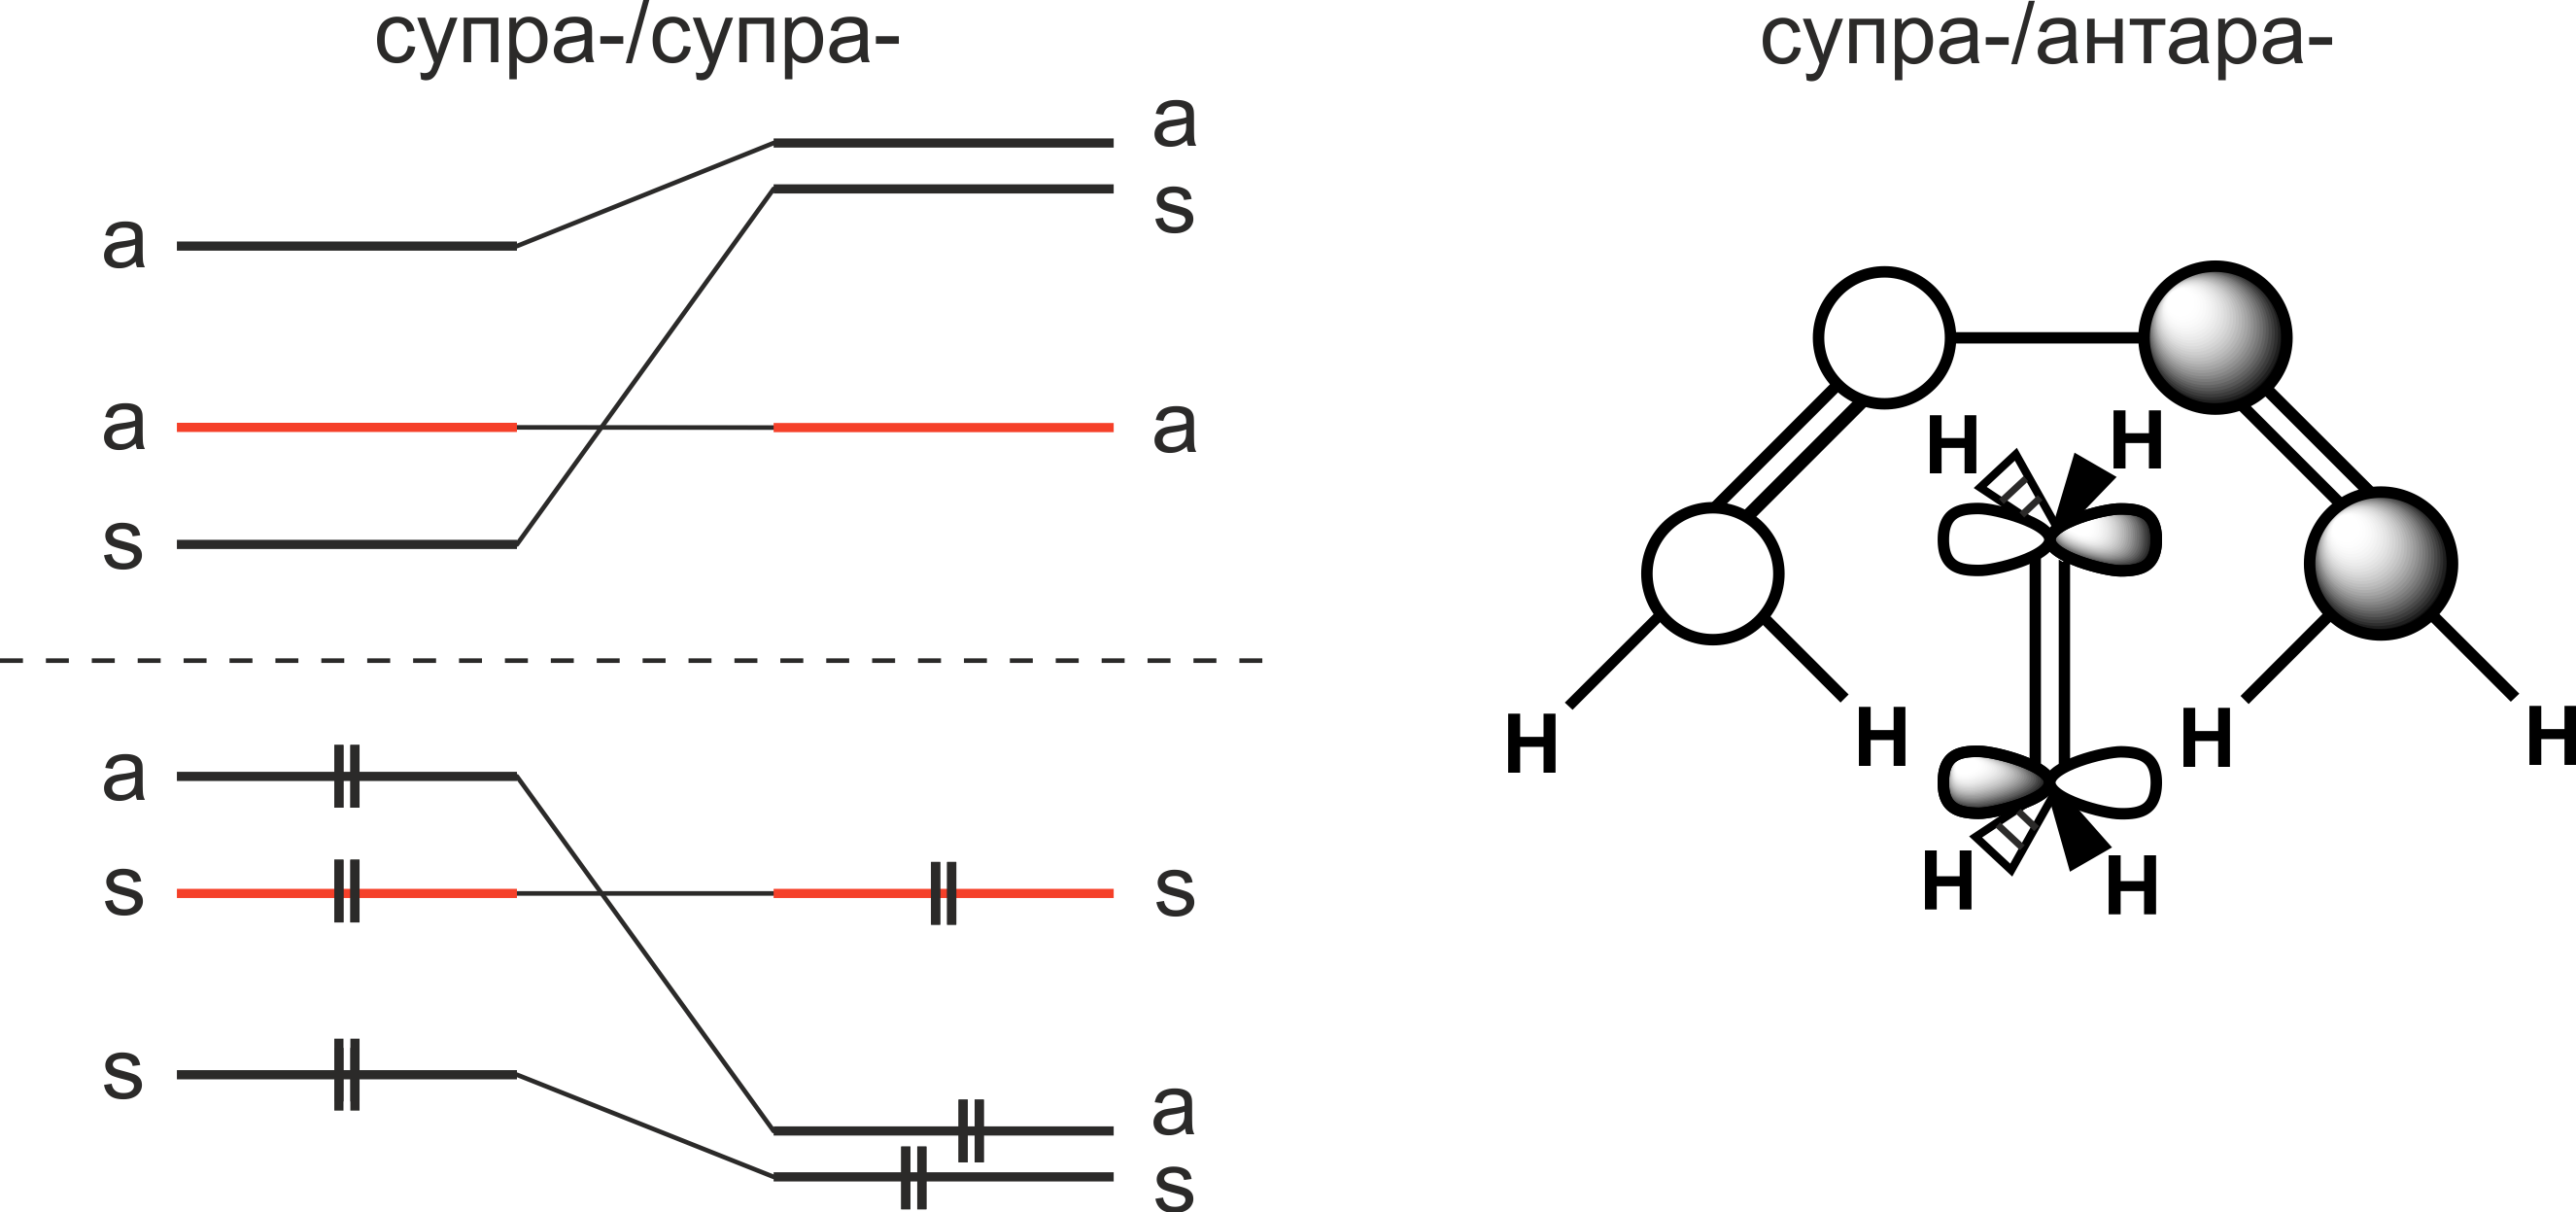
\includegraphics[width=6.5cm]{images/Fig_2_1_4_dec.png}
\centering
\end{figure}
\vspace{-\parskip}
\par
\begin{wrapfigure}{r}{30mm} %this figure will be at the right
    \centering
    \vspace{-0.7mm}
    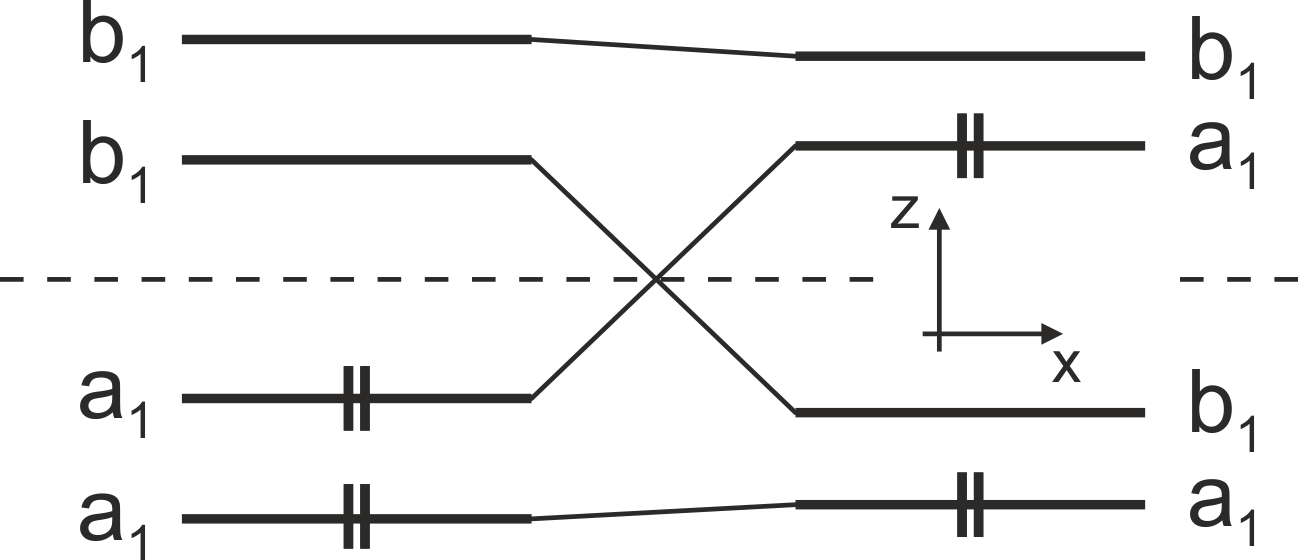
\includegraphics[width=30mm]{images/Fig_2_1_5_dec.png}
    \vspace{-9mm}
\end{wrapfigure}
5. В ходе всей реакции сохраняется группа симметрии  $C_{2v}$. Реакция протекает фотохимически. Корреляционная диаграмма приведена на рисунке.\par
%\vspace{-\parskip}
\begin{wrapfigure}{r}{30mm} %this figure will be at the right
    \centering
    \vspace{5.4mm}
    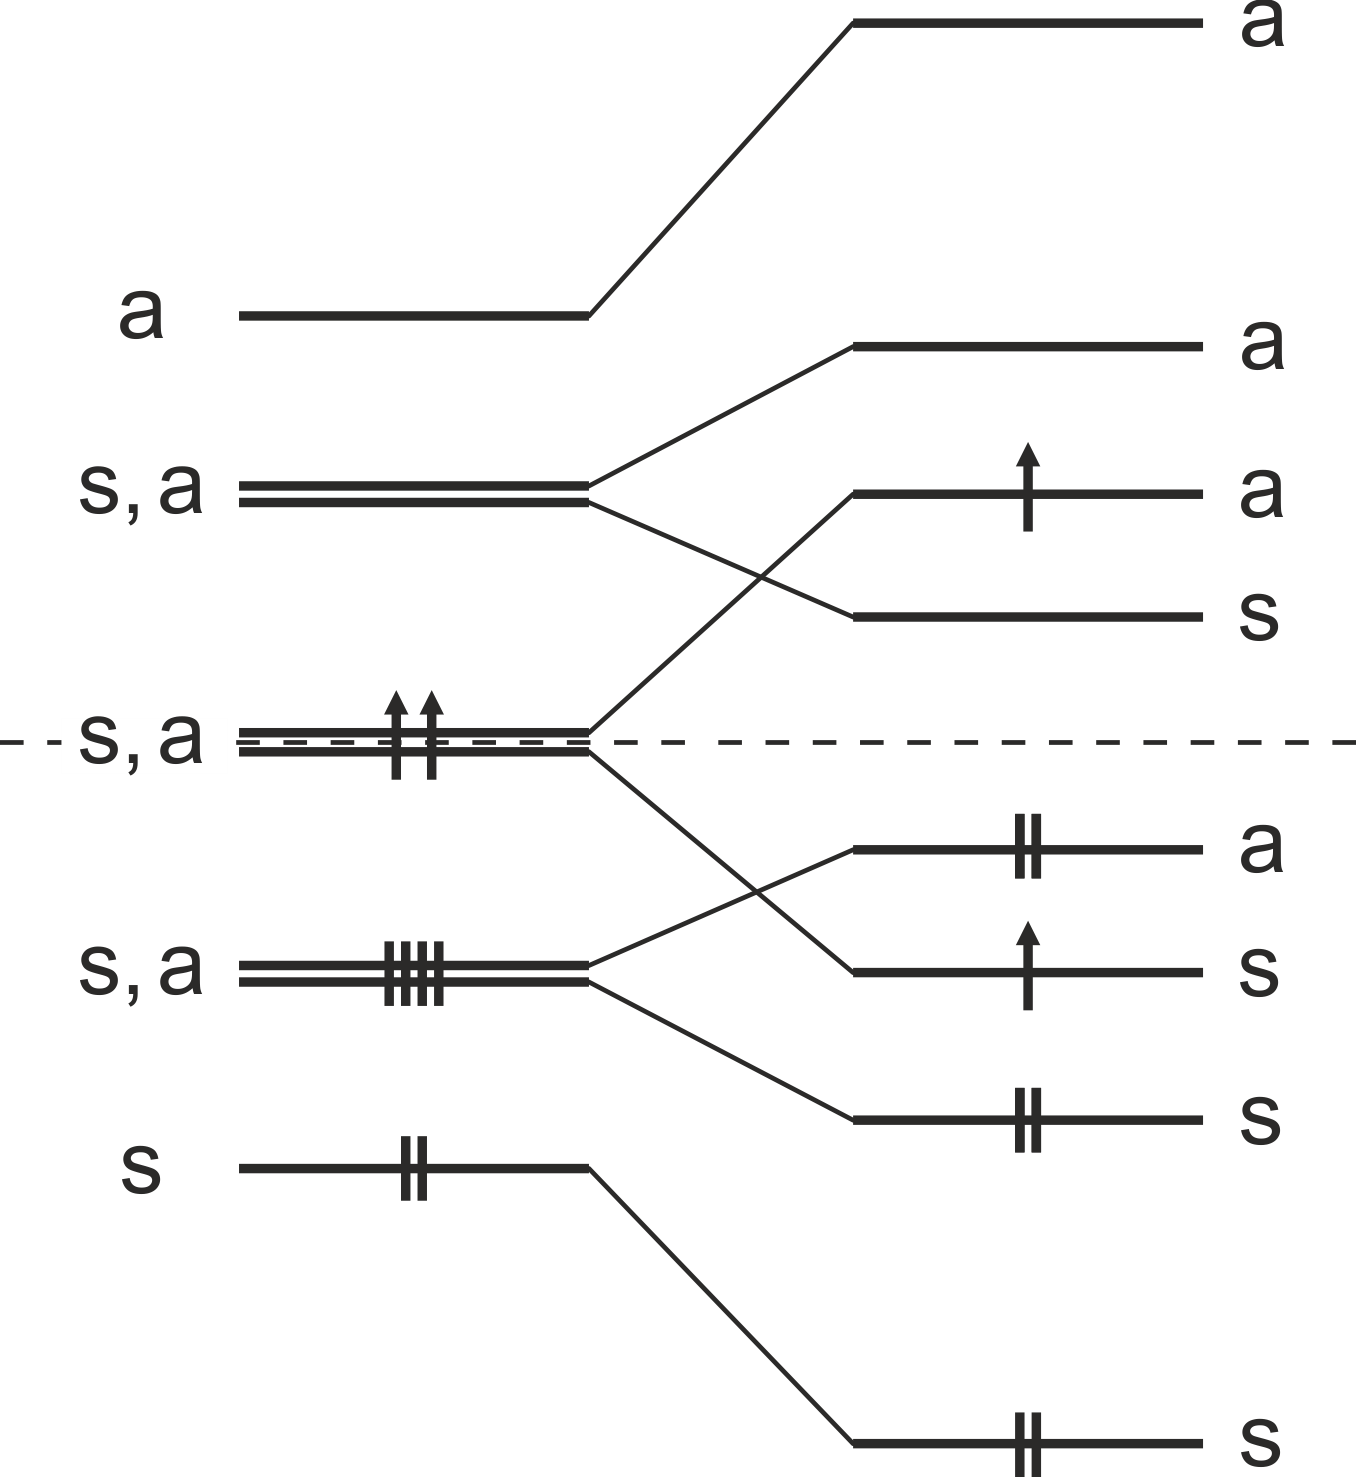
\includegraphics[width=30mm]{images/Fig_2_1_6_dec.png}
    \vspace{-5mm}
\end{wrapfigure}
6. Если считать, что циклооктатетраен плоский, то его основной терм триплетный по спину и реакция запрещена термически для дисротаторного механизма. Корреляционная диаграмма приведена на рисунке. Данный подход не совсем корректный. Если же учесть конформацию циклооктатетраена, необходимую для протекация реакции, то данная реакция в дисротаторном механизме соответствует трем $2\pi_s$ компонентам, то~есть она разрешена термически. В этом случае одна двойная связь выходит из сопряжения и~не участвует в~реакции. Реагент необходимо рассматривать как две линейные $\pi$-системы из 2 и 6 атомов, соответственно.\par
%\vspace{-\parskip}
\begin{wrapfigure}{r}{30mm} %this figure will be at the right
    \centering
    \vspace{-1mm}
    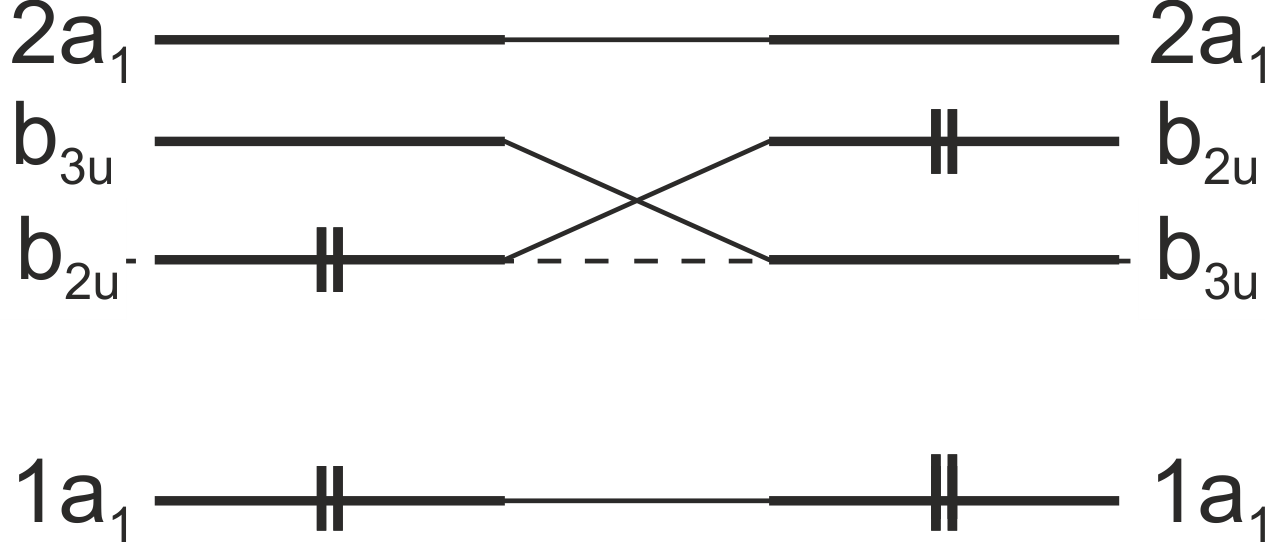
\includegraphics[width=30mm]{images/Fig_2_1_7_dec.png}
    \vspace{-5mm}
\end{wrapfigure}
7. В ходе всей реакции сохраняется группа симметрии $D_{2h}$. Корреляционная диаграмма для указанной в~условии системы координат и базиса $1s$ атомных орбиталей приведена на рисунке, реакция запрещена термически. Изменение полной электронной энергии равно $-2\beta$.\par
%\vspace{-\parskip}
8. Общая формулировка правил Вудворда-Хоффмана: перициклическая реакция термически разрешена если общее число $4n+2$ супраповерхностых и~$4n$~антараповерхностных компонент равно нечетному числу.  Более конкретно для~циклоприсоединения Дильса-Альдера, если $p+q=4n$, то реакция разрешена термически для супра-/антара- и антара-/супра- топологий, разрешена фотохимически для супра-/супра- и антара-/антара- топологий. Если $p+q=4n+2$, то~реакция разрешена термически для супра-/супра- и антара-/антара- топологий, разрешена фотохимически для супра-/антара- и антара-/супра- топологий. В~данном случае $p$ и $q$ равны количеству электронов в $\pi$-системах реагентов, а~$n$~– целое число.\par
%\vspace{-\parskip}
\begin{wrapfigure}{r}{30mm} %this figure will be at the right
    \centering
    \vspace{0mm}
    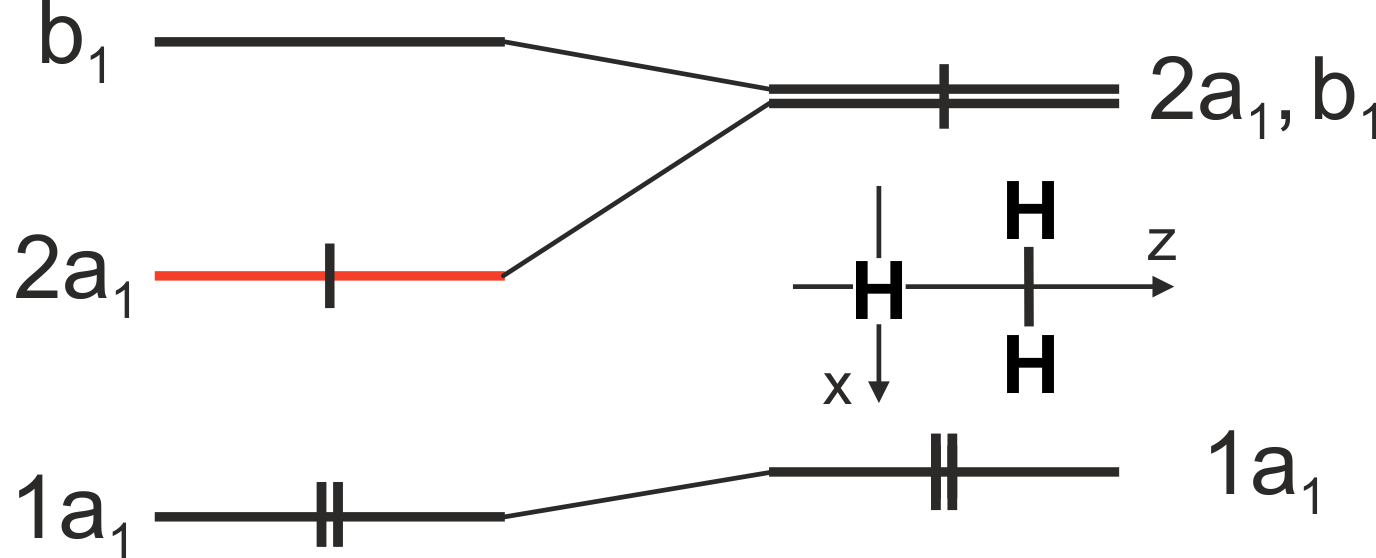
\includegraphics[width=30mm]{images/Fig_2_1_9_dec.png}
    \vspace{-5mm}
\end{wrapfigure}
9. В ходе всей реакции сохраняется группа симметрии $C_{2v}$. Корреляционная диаграмма приведена на рисунке. Реакция разрешена термически. Электрический дипольный переход в~H$_2$ возможен в конфигурацию $a_1^1b_1^1$, терм $^1B_1$. Фотохимически реакция также разрешена.\par
%\vspace{-\parskip}
10. Данная рекция может протекать как через промежуточное состояние в~конформации кресло, так и в конформации ванна. Рассмотрим для определенности только конформацию кресло. Как показано на рисунке, в этом случае реакция соответствует $2\pi_s$ + $2\pi_s$ + $2\sigma_s$ компонентам. Всего три $4n+2$ супра-компоненты, то есть реакция разрешена термически. Стереохимия продукта также приведена на рисунке. В случае конформации ванна данная реакция также разрешена термически.\par
\vspace{-\parskip}
\vspace{1mm}
\begin{figure}[h]
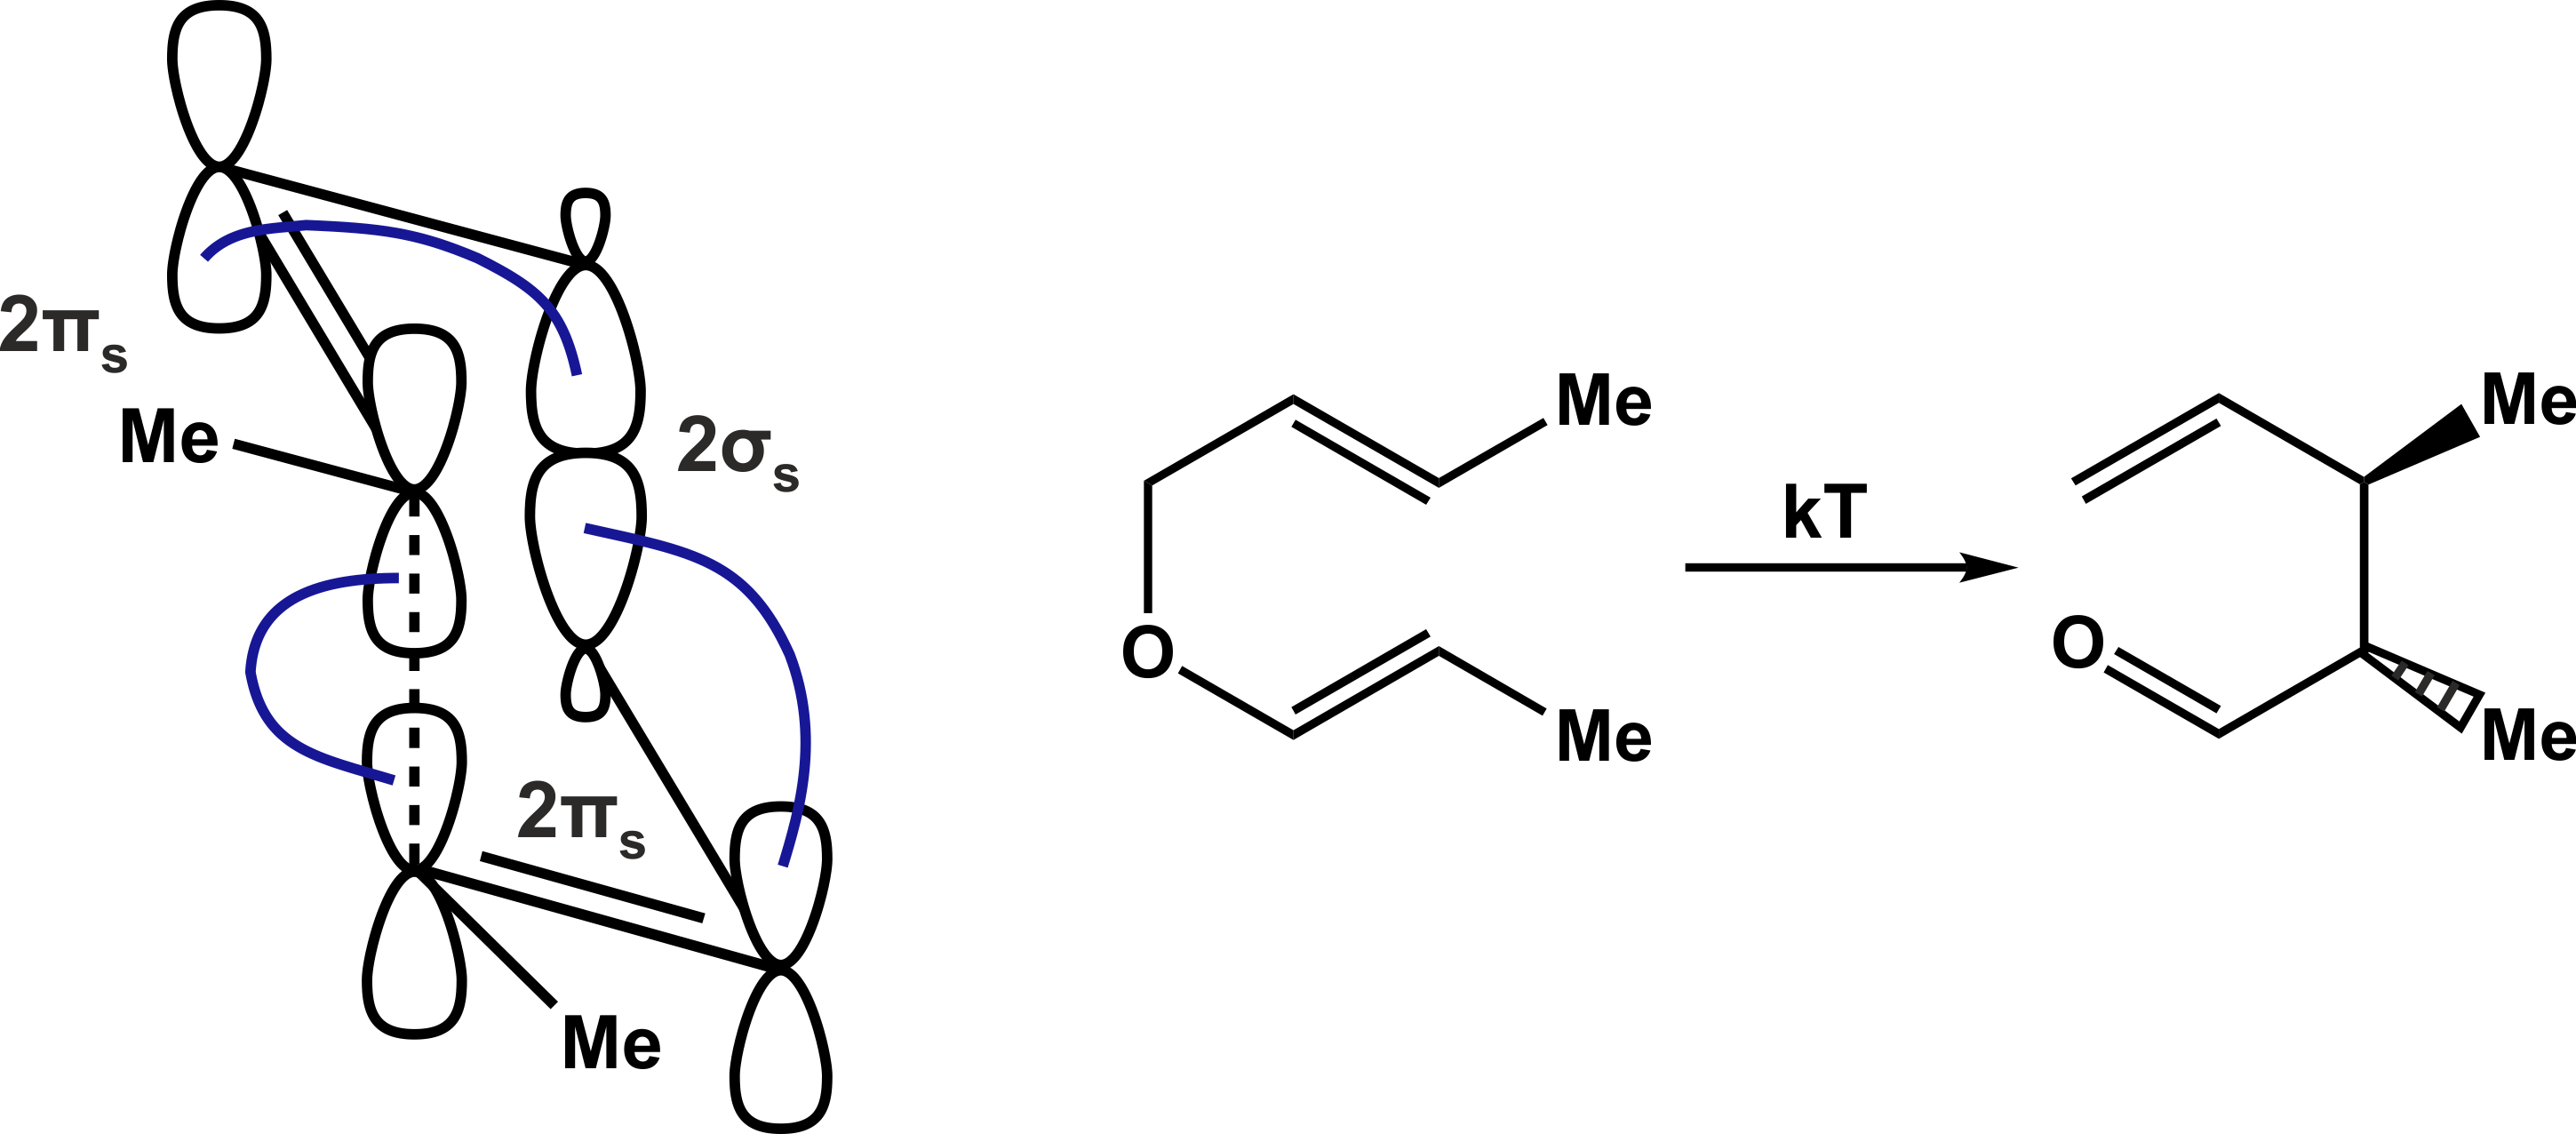
\includegraphics[width=6.5cm]{images/Fig_2_1_10_dec.png}
\centering
\end{figure}
\par
%\vspace{-\parskip}
\vspace{-\parskip}
\begin{wrapfigure}{r}{30mm} %this figure will be at the right
    \centering
    \vspace{4mm}
    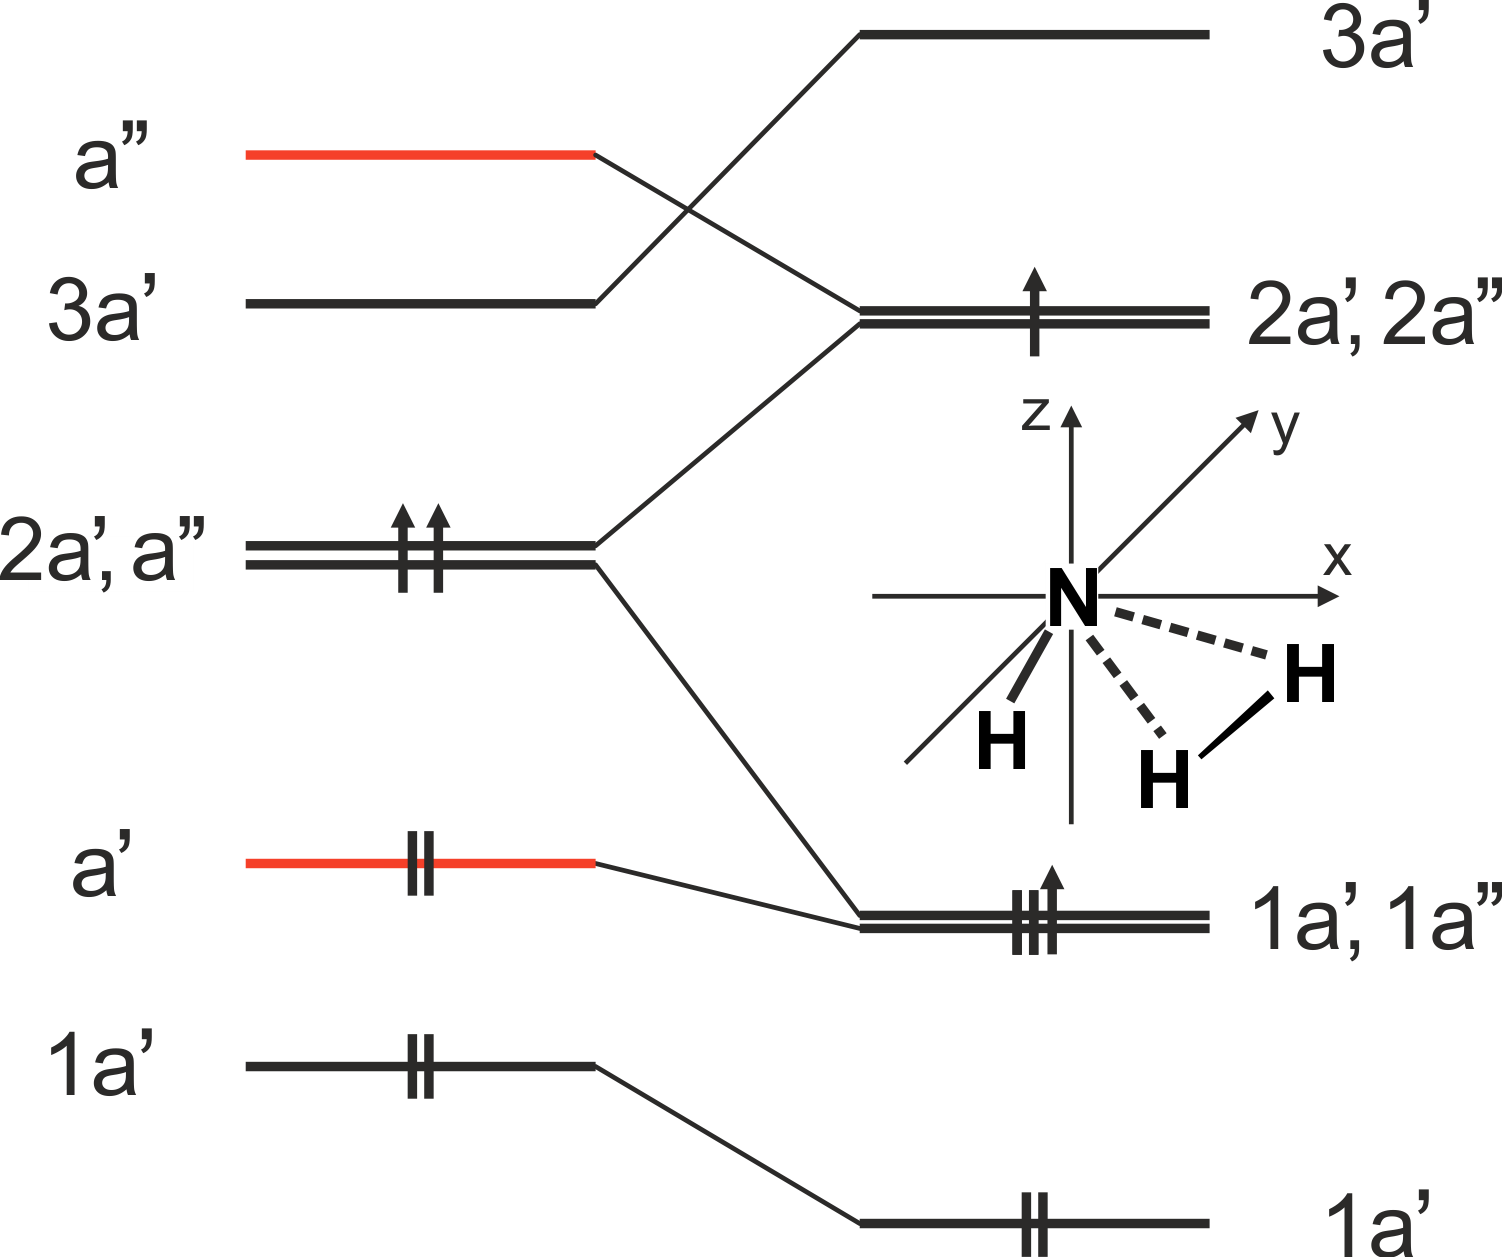
\includegraphics[width=30mm]{images/Fig_2_1_11_dec.png}
    \vspace{-5mm}
\end{wrapfigure}
11. В ходе всей реакции сохраняется группа симметрии $C_s$ с единственной операцией симметриии $\sigma_{zx}$. Корреляционная диаграмма приведена на рисунке. Для простоты для атома азота учитываются только $2p$ атомные орбитали. Расположение молекулярных орбиталей по~энергии приведено качественно. Молекулярные орбитали молекулы водорода выделены красным цветом. Основное триплетное состояние реагентов коррелирует с возбужденным состоянием молекулы аммиака. Реакция запрещена термически.\par
12. Считаем, что при таком протекании реакции $3d$ атомные орбитали металла включены в систему молекулярных орбиталей. Их расщепление в поле двух этиленов для простоты не учитываем. В ходе всей реакции сохраняется группа симметрии $C_{2v}$. Корреляционная диаграмма приведена на рисунке. Реакция термически разрешена для электронных конфигураций $3d^2-3d^8$, без учета спиновой мультиплетности основного терма металла.\par
\vspace{-\parskip}
\vspace{1.5mm}
\begin{figure}[h]
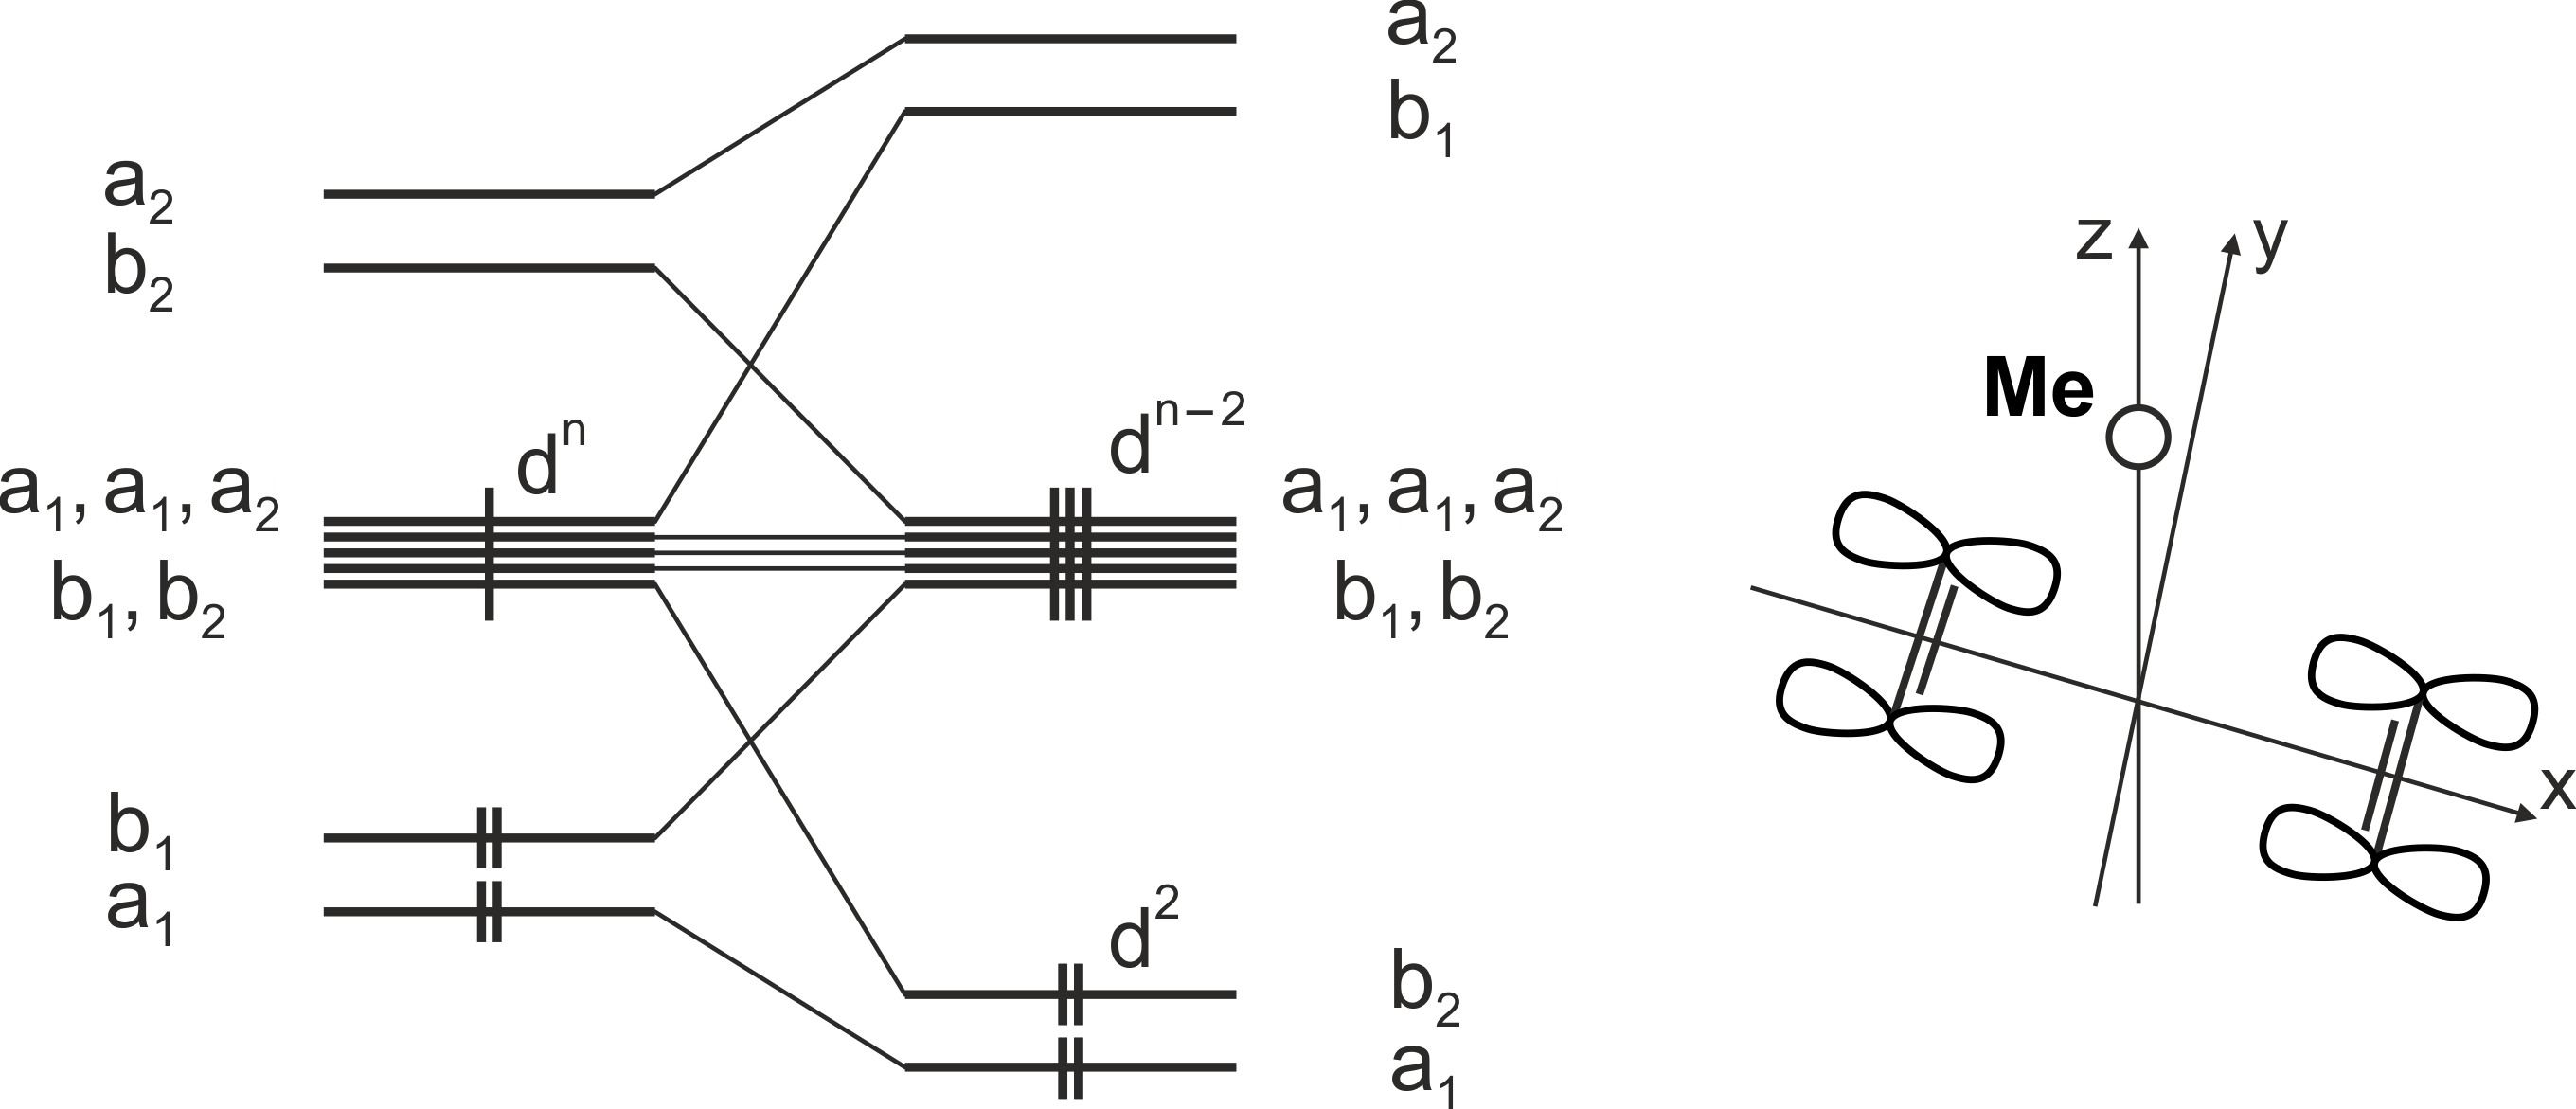
\includegraphics[width=6.5cm]{images/Fig_2_1_12_dec.png}
\centering
\end{figure}
\par
13. Задача 2 контрольной работы 1 весеннего семестра 2024/2025 учебного года. Корреляционная диаграмма для супра-/супра- топологии приведена на~рисунке ниже.
\vspace{-\parskip}
\vspace{1.5mm}
\begin{figure}[h]
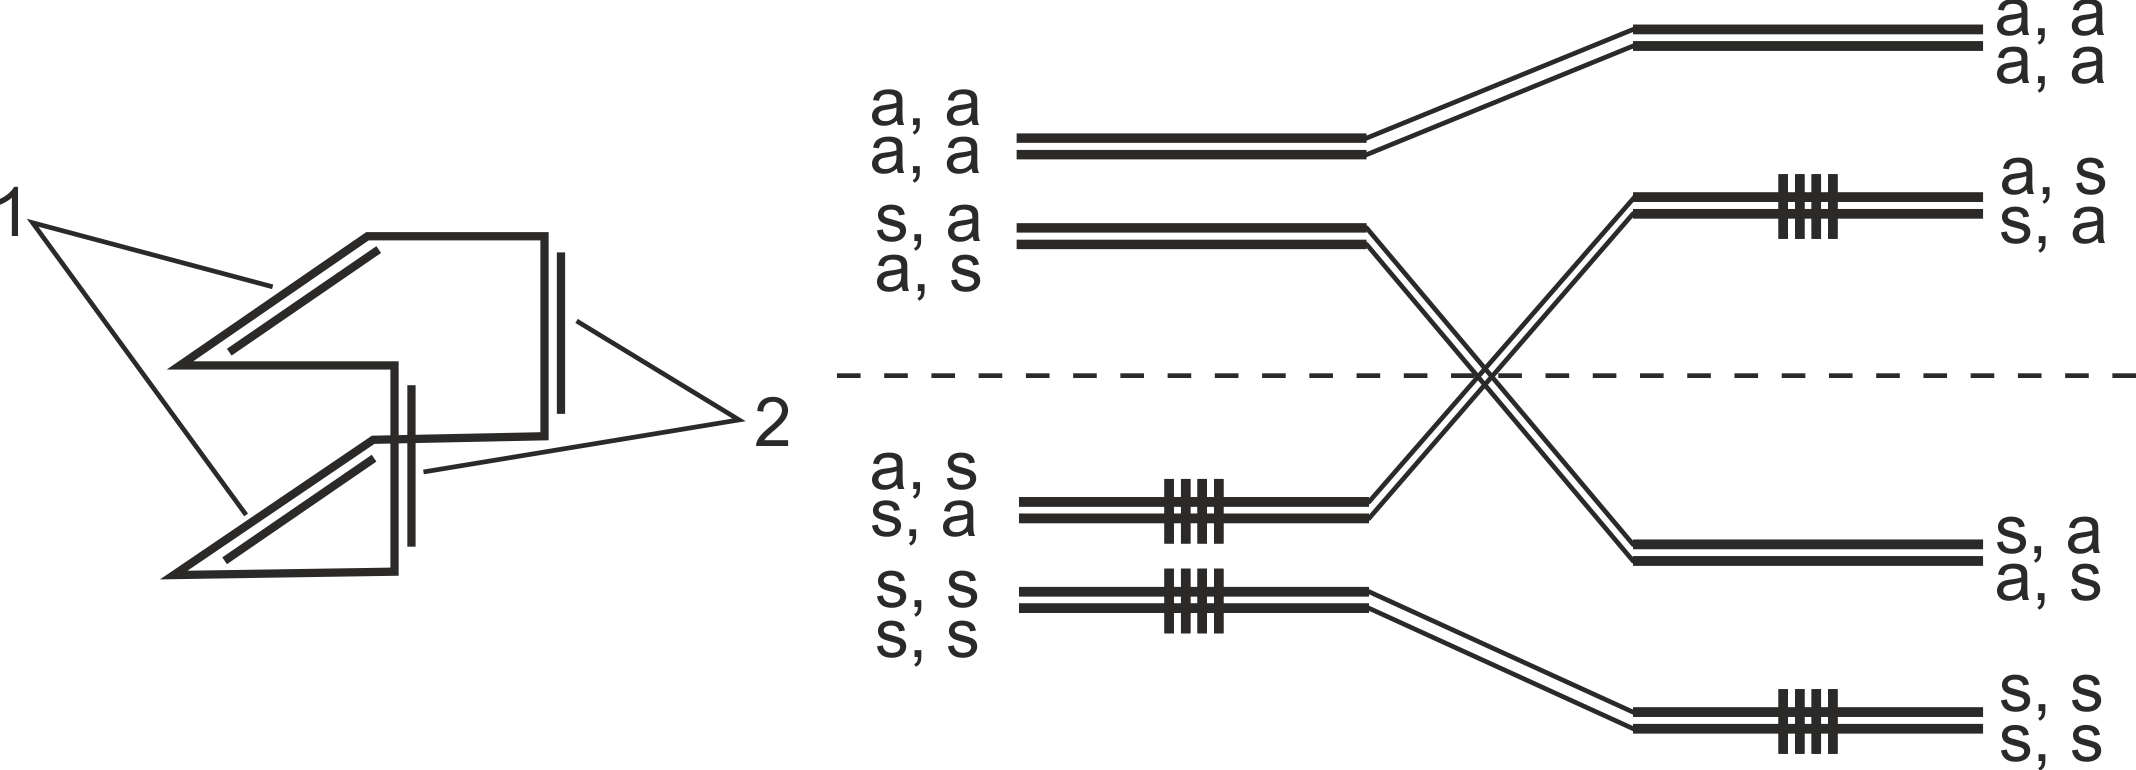
\includegraphics[width=8cm]{images/Fig_2_1_13_dec.png}
\centering
\end{figure}
\par
\vspace{-\parskip}
\newpage

\subsection{Теория кристаллического поля}
1. \\
2. 
\newpage

\subsection{Электронная спектроскопия}
1. \\
2. 
\newpage

\subsection{ИК и КР спектроскопии}
1. \\
2. 
\newpage

\subsection{Эффект Яна-Теллера}
1. \\
2. 
\newpage

\subsection{Вращательная спектроскопия и ее производные}
1. Предел канта равен $\frac{\text{d}}{\text{d}J}( \Delta E_R) = -\frac{1}{2}-\frac{B'}{B'-B}$, где $B'$ и $B$ – вращательные постоянные для колебательных состояний $\nu=1$ и $\nu=0$, соответственно. Подстановка межъядерного расстояния в эту формулу после округления до ближайшего целого числа дает 49.\par
2. $B=6,08114$ ГГц, $I=1,37\cdot10^{-45}$ кг$\cdot$м$^2$. Длины связей определяются из системы уравнений, составленной на основе моментов инерции изотопологов $^{16}\text{O}^{12}\text{C}^{32}\text{S}$ и~$^{16}\text{O}^{12}\text{C}^{34}\text{S}$, посчитанных с помощью приведенных в~условии данных.\par
3. \par
4. Группа симметрии $D_{4h}$, симметрический волчок. $A=B/2$.\par
5. X$-$X$-$Y линейная.\par
6. $J=2k$, $F=0$; $J=2k+1$, $F=1$, где $F$ – полный ядерный спин двух атомов водорода, $k$ – положительное целое число.\par
7. \par
8. \par
9. 25/64.\par
10. \par
11. Задача 2 контрольной работы 2 весеннего семестра 2024/2025 учебного года. $R=1,25\cdot10^{-10}$ м. Молекула HCl имеет приведенную массу, близкую к заданной в условии. \par
12. Задача 2 контрольной работы 2 весеннего семестра 2023/2024 учебного года. $B=3013,845$ МГц, $R=2,17\cdot10^{-10}$ м.\par
13. Задача 2 контрольной работы 2 весеннего семестра 2022/2023 учебного года. В обоих случаях чисто вращательный спектр будет представлять из себя набор эквидистантных линий, с расстоянием между линиями равным вращательной постоянной и относительной интенсивностью, определяемой населенностью вращательных уровней $N_J$. Населенность равна $(2J+1)\exp(-BJ(J+1)/kT)$ и~$(J+1)\exp(-BJ(J+1)/kT)$, соответственно, без учета и при учете описанного в~условии фактора. Анализ показывает, что максимум указанных величин $N_J$~достигается при $J_{max}\approx 2,65$ и $J_{max}\approx 2,41$. Таким образом, максимальной интенсивности будут обадать линии, соответствующие переходам с вращательных уровней $J=2$ и $J=3$.\par
\newpage

\subsection{ЭПР спектроскопия}
1. \\
2. 
\newpage

\subsection{Химический обмен в магнитном резонансе}
1. \\
2. 
\newpage

\subsection{ЯМР спектроскопия}
1. \\
2. 
\newpage
